\documentclass[twoside]{article}

% Packages required by doxygen
\usepackage{calc}
\usepackage{doxygen}
\usepackage{graphicx}
\usepackage[utf8]{inputenc}
\usepackage{makeidx}
\usepackage{multicol}
\usepackage{multirow}
\usepackage{textcomp}
\usepackage[table]{xcolor}

% Font selection
\usepackage[T1]{fontenc}
\usepackage{mathptmx}
\usepackage[scaled=.90]{helvet}
\usepackage{courier}
\usepackage{amssymb}
\usepackage{sectsty}
\renewcommand{\familydefault}{\sfdefault}
\allsectionsfont{%
  \fontseries{bc}\selectfont%
  \color{darkgray}%
}
\renewcommand{\DoxyLabelFont}{%
  \fontseries{bc}\selectfont%
  \color{darkgray}%
}

% Page & text layout
\usepackage{geometry}
\geometry{%
  letterpaper,%
  top=2.5cm,%
  bottom=2.5cm,%
  left=2.5cm,%
  right=2.5cm%
}
\tolerance=750
\hfuzz=15pt
\hbadness=750
\setlength{\emergencystretch}{15pt}
\setlength{\parindent}{0cm}
\setlength{\parskip}{0.2cm}
\makeatletter
\renewcommand{\paragraph}{%
  \@startsection{paragraph}{4}{0ex}{-1.0ex}{1.0ex}{%
    \normalfont\normalsize\bfseries\SS@parafont%
  }%
}
\renewcommand{\subparagraph}{%
  \@startsection{subparagraph}{5}{0ex}{-1.0ex}{1.0ex}{%
    \normalfont\normalsize\bfseries\SS@subparafont%
  }%
}
\makeatother

% Headers & footers
\usepackage{fancyhdr}
\pagestyle{fancyplain}
\fancyhead[LE]{\fancyplain{}{\bfseries\thepage}}
\fancyhead[CE]{\fancyplain{}{}}
\fancyhead[RE]{\fancyplain{}{\bfseries\leftmark}}
\fancyhead[LO]{\fancyplain{}{\bfseries\rightmark}}
\fancyhead[CO]{\fancyplain{}{}}
\fancyhead[RO]{\fancyplain{}{\bfseries\thepage}}
\fancyfoot[LE]{\fancyplain{}{}}
\fancyfoot[CE]{\fancyplain{}{}}
\fancyfoot[RE]{\fancyplain{}{\bfseries\scriptsize Generated on Sun Apr 26 2015 18\-:16\-:07 for Motorcycle Awareness System (\-M\-A\-S) by Doxygen }}
\fancyfoot[LO]{\fancyplain{}{\bfseries\scriptsize Generated on Sun Apr 26 2015 18\-:16\-:07 for Motorcycle Awareness System (\-M\-A\-S) by Doxygen }}
\fancyfoot[CO]{\fancyplain{}{}}
\fancyfoot[RO]{\fancyplain{}{}}
\renewcommand{\footrulewidth}{0.4pt}
\renewcommand{\sectionmark}[1]{%
  \markright{\thesection\ #1}%
}

% Indices & bibliography
\usepackage{natbib}
\usepackage[titles]{tocloft}
\setcounter{tocdepth}{3}
\setcounter{secnumdepth}{5}
\makeindex

% Hyperlinks (required, but should be loaded last)
\usepackage{ifpdf}
\ifpdf
  \usepackage[pdftex,pagebackref=true]{hyperref}
\else
  \usepackage[ps2pdf,pagebackref=true]{hyperref}
\fi
\hypersetup{%
  colorlinks=true,%
  linkcolor=blue,%
  citecolor=blue,%
  unicode%
}

% Custom commands
\newcommand{\clearemptydoublepage}{%
  \newpage{\pagestyle{empty}\cleardoublepage}%
}


%===== C O N T E N T S =====

\begin{document}

% Titlepage & ToC
\hypersetup{pageanchor=false}
\pagenumbering{roman}
\begin{titlepage}
\vspace*{7cm}
\begin{center}%
{\Large Motorcycle Awareness System (M\-A\-S) \\[1ex]\large M\-E553 Group E\-P\-E 6 }\\
\vspace*{1cm}
{\large Generated by Doxygen 1.8.6}\\
\vspace*{0.5cm}
{\small Sun Apr 26 2015 18:16:07}\\
\end{center}
\end{titlepage}
\tableofcontents
\pagenumbering{arabic}
\hypersetup{pageanchor=true}

%--- Begin generated contents ---
\section{Motorcycle Awareness System Overview}
\label{index}\hypertarget{index}{}This low-\/level design documentation details a mockup of the Motorcycle Awareness System. It provides part of the functionality of the M\-A\-S for both the motorcycle and car. Mocking of input signals such as the radar signals, vehicle-\/to-\/vehicle (V2\-V) communication signals, and G\-P\-S signals mimics the interactions that the M\-A\-S would have with actual sensor data on the finished product.

The implemented functionality includes continuous tracking of the motorcycle using G\-P\-S, determining whether a hazard is present using the motorcycle's radar sensor signals, and relaying a warning to the motorcycle rider of a potential threat. For the car, the logic determines whether the car's blinker is on based on blinker signal data on the C\-A\-N bus, determines whether a motorcycle is in range and assess the potential danger, and issues a warning to the driver as necessary.

{\bfseries M\-A\-S Concept Sketch}  
\begin{DoxyImage}
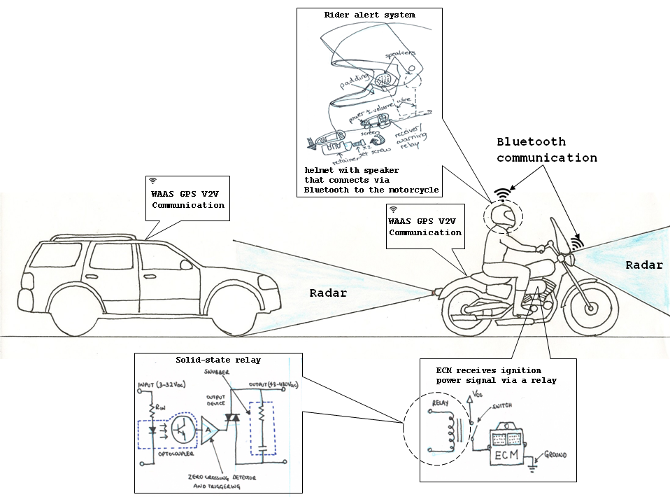
\includegraphics[width=12cm]{MAS_system_overview}
\caption{M\-A\-S concept sketch}
\end{DoxyImage}
 
\section{Todo List}
\label{todo}
\hypertarget{todo}{}

\begin{DoxyRefList}
\item[\label{todo__todo000003}%
\hypertarget{todo__todo000003}{}%
Member \hyperlink{classMotorcycleAwarenessSystem_a840a5bc17d75276ecdb3a39d7aaf4109}{Motorcycle\-Awareness\-System\-:\-:Get\-Motorcycle\-Location} (void)]Acquire the data packet from the motorcycle  
\item[\label{todo__todo000001}%
\hypertarget{todo__todo000001}{}%
Member \hyperlink{classMotorcycleAwarenessSystem_a239655aca9c875b1dbbad3ce155c7892}{Motorcycle\-Awareness\-System\-:\-:Is\-Motorcycle\-In\-Range} (void)]Process the data packet and determine threat  
\item[\label{todo__todo000002}%
\hypertarget{todo__todo000002}{}%
Member \hyperlink{classMotorcycleAwarenessSystem_aec5e4731c6bf0789821ba2793918e3ee}{Motorcycle\-Awareness\-System\-:\-:Relay\-Warning\-To\-Operator} (void)]Transmit the bluetooth message to the operator 
\end{DoxyRefList}
\section{Class Index}
\subsection{Class List}
Here are the classes, structs, unions and interfaces with brief descriptions\-:\begin{DoxyCompactList}
\item\contentsline{section}{\hyperlink{structBlueToothMessage__t}{Blue\-Tooth\-Message\-\_\-t} \\*Struct for bluetooth message }{\pageref{structBlueToothMessage__t}}{}
\item\contentsline{section}{\hyperlink{structGpsSignal__t}{Gps\-Signal\-\_\-t} \\*Structure that emulates a G\-P\-S signal }{\pageref{structGpsSignal__t}}{}
\item\contentsline{section}{\hyperlink{classMotorcycleAwarenessSystem}{Motorcycle\-Awareness\-System} \\*Class declaration for the Motorcycle Awareness System (M\-A\-S) }{\pageref{classMotorcycleAwarenessSystem}}{}
\item\contentsline{section}{\hyperlink{structMotorCycleLocation__t}{Motor\-Cycle\-Location\-\_\-t} \\*Struct for the V2\-V data }{\pageref{structMotorCycleLocation__t}}{}
\item\contentsline{section}{\hyperlink{structRadarSignal__t}{Radar\-Signal\-\_\-t} \\*Structure that emulates a Radar signal }{\pageref{structRadarSignal__t}}{}
\item\contentsline{section}{\hyperlink{structTurnSignal__t}{Turn\-Signal\-\_\-t} }{\pageref{structTurnSignal__t}}{}
\end{DoxyCompactList}

\section{File Index}
\subsection{File List}
Here is a list of all files with brief descriptions\-:\begin{DoxyCompactList}
\item\contentsline{section}{\hyperlink{main_8cpp}{main.\-cpp} }{\pageref{main_8cpp}}{}
\item\contentsline{section}{\hyperlink{MotorcycleAwarenessSystem_8cpp}{Motorcycle\-Awareness\-System.\-cpp} }{\pageref{MotorcycleAwarenessSystem_8cpp}}{}
\item\contentsline{section}{\hyperlink{MotorcycleAwarenessSystem_8hpp}{Motorcycle\-Awareness\-System.\-hpp} }{\pageref{MotorcycleAwarenessSystem_8hpp}}{}
\item\contentsline{section}{\hyperlink{MotorcycleAwarenessSystemTypes_8hpp}{Motorcycle\-Awareness\-System\-Types.\-hpp} }{\pageref{MotorcycleAwarenessSystemTypes_8hpp}}{}
\end{DoxyCompactList}

\section{Class Documentation}
\hypertarget{structBlueToothMessage__t}{\section{Blue\-Tooth\-Message\-\_\-t Struct Reference}
\label{structBlueToothMessage__t}\index{Blue\-Tooth\-Message\-\_\-t@{Blue\-Tooth\-Message\-\_\-t}}
}


Struct for bluetooth message.  




{\ttfamily \#include $<$Motorcycle\-Awareness\-System\-Types.\-hpp$>$}



Collaboration diagram for Blue\-Tooth\-Message\-\_\-t\-:\nopagebreak
\begin{figure}[H]
\begin{center}
\leavevmode
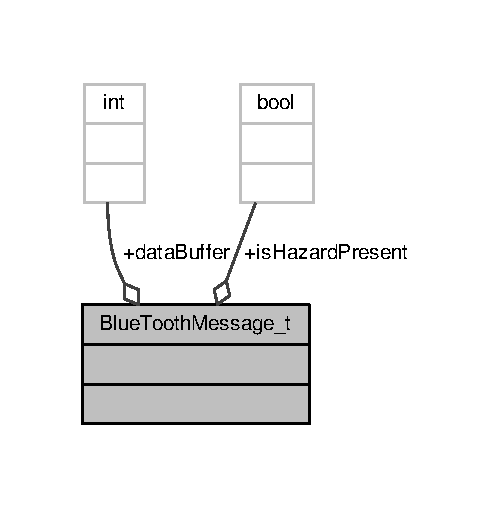
\includegraphics[width=236pt]{structBlueToothMessage__t__coll__graph}
\end{center}
\end{figure}
\subsection*{Public Attributes}
\begin{DoxyCompactItemize}
\item 
bool \hyperlink{structBlueToothMessage__t_a2dd315aa1cba1d2d3045e26b9f171e61}{is\-Hazard\-Present}
\begin{DoxyCompactList}\small\item\em Hazard flag. \end{DoxyCompactList}\item 
unsigned int \hyperlink{structBlueToothMessage__t_ab872789a32f068dae8bcf77122256b78}{data\-Buffer} \mbox{[}255\mbox{]}
\begin{DoxyCompactList}\small\item\em Bluetooth data buffer. \end{DoxyCompactList}\end{DoxyCompactItemize}


\subsection{Detailed Description}
Struct for bluetooth message. 

Definition at line \hyperlink{MotorcycleAwarenessSystemTypes_8hpp_source_l00041}{41} of file \hyperlink{MotorcycleAwarenessSystemTypes_8hpp_source}{Motorcycle\-Awareness\-System\-Types.\-hpp}.



\subsection{Member Data Documentation}
\hypertarget{structBlueToothMessage__t_ab872789a32f068dae8bcf77122256b78}{\index{Blue\-Tooth\-Message\-\_\-t@{Blue\-Tooth\-Message\-\_\-t}!data\-Buffer@{data\-Buffer}}
\index{data\-Buffer@{data\-Buffer}!BlueToothMessage_t@{Blue\-Tooth\-Message\-\_\-t}}
\subsubsection[{data\-Buffer}]{\setlength{\rightskip}{0pt plus 5cm}unsigned int Blue\-Tooth\-Message\-\_\-t\-::data\-Buffer\mbox{[}255\mbox{]}}}\label{structBlueToothMessage__t_ab872789a32f068dae8bcf77122256b78}


Bluetooth data buffer. 



Definition at line \hyperlink{MotorcycleAwarenessSystemTypes_8hpp_source_l00044}{44} of file \hyperlink{MotorcycleAwarenessSystemTypes_8hpp_source}{Motorcycle\-Awareness\-System\-Types.\-hpp}.

\hypertarget{structBlueToothMessage__t_a2dd315aa1cba1d2d3045e26b9f171e61}{\index{Blue\-Tooth\-Message\-\_\-t@{Blue\-Tooth\-Message\-\_\-t}!is\-Hazard\-Present@{is\-Hazard\-Present}}
\index{is\-Hazard\-Present@{is\-Hazard\-Present}!BlueToothMessage_t@{Blue\-Tooth\-Message\-\_\-t}}
\subsubsection[{is\-Hazard\-Present}]{\setlength{\rightskip}{0pt plus 5cm}bool Blue\-Tooth\-Message\-\_\-t\-::is\-Hazard\-Present}}\label{structBlueToothMessage__t_a2dd315aa1cba1d2d3045e26b9f171e61}


Hazard flag. 



Definition at line \hyperlink{MotorcycleAwarenessSystemTypes_8hpp_source_l00043}{43} of file \hyperlink{MotorcycleAwarenessSystemTypes_8hpp_source}{Motorcycle\-Awareness\-System\-Types.\-hpp}.



The documentation for this struct was generated from the following file\-:\begin{DoxyCompactItemize}
\item 
\hyperlink{MotorcycleAwarenessSystemTypes_8hpp}{Motorcycle\-Awareness\-System\-Types.\-hpp}\end{DoxyCompactItemize}

\hypertarget{structGpsSignal__t}{\subsection{Gps\-Signal\-\_\-t Struct Reference}
\label{structGpsSignal__t}\index{Gps\-Signal\-\_\-t@{Gps\-Signal\-\_\-t}}
}


Structure that emulates a G\-P\-S signal.  




{\ttfamily \#include $<$Motorcycle\-Awareness\-System\-Types.\-hpp$>$}



Collaboration diagram for Gps\-Signal\-\_\-t\-:\nopagebreak
\begin{figure}[H]
\begin{center}
\leavevmode
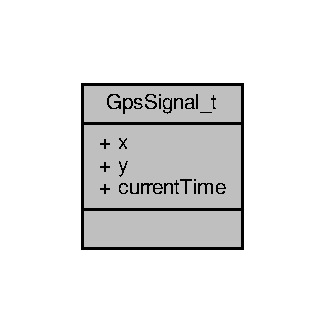
\includegraphics[width=176pt]{structGpsSignal__t__coll__graph}
\end{center}
\end{figure}
\subsubsection*{Public Attributes}
\begin{DoxyCompactItemize}
\item 
\hyperlink{MotorcycleAwarenessSystemTypes_8hpp_ae989615510617e9b0ad39dcd343c78fb}{Coordinate\-\_\-t} \hyperlink{structGpsSignal__t_a6f7bd3c500b55923ab335ada4b6b26eb}{x}
\begin{DoxyCompactList}\small\item\em x-\/axis coordinate \end{DoxyCompactList}\item 
\hyperlink{MotorcycleAwarenessSystemTypes_8hpp_ae989615510617e9b0ad39dcd343c78fb}{Coordinate\-\_\-t} \hyperlink{structGpsSignal__t_ab9e083be189fc842ed7aa4fdc978e94e}{y}
\begin{DoxyCompactList}\small\item\em y-\/axis coordinate \end{DoxyCompactList}\item 
\hyperlink{MotorcycleAwarenessSystemTypes_8hpp_a75ae168a2dad22557428f696df806a76}{current\-Time\-\_\-t} \hyperlink{structGpsSignal__t_abc96245129f39c6e51e8bfe955f2047e}{current\-Time}
\begin{DoxyCompactList}\small\item\em Current time at coordinates x,y. \end{DoxyCompactList}\end{DoxyCompactItemize}


\subsubsection{Detailed Description}
Structure that emulates a G\-P\-S signal. 

Definition at line \hyperlink{MotorcycleAwarenessSystemTypes_8hpp_source_l00025}{25} of file \hyperlink{MotorcycleAwarenessSystemTypes_8hpp_source}{Motorcycle\-Awareness\-System\-Types.\-hpp}.



\subsubsection{Member Data Documentation}
\hypertarget{structGpsSignal__t_abc96245129f39c6e51e8bfe955f2047e}{\index{Gps\-Signal\-\_\-t@{Gps\-Signal\-\_\-t}!current\-Time@{current\-Time}}
\index{current\-Time@{current\-Time}!GpsSignal_t@{Gps\-Signal\-\_\-t}}
\paragraph[{current\-Time}]{\setlength{\rightskip}{0pt plus 5cm}{\bf current\-Time\-\_\-t} Gps\-Signal\-\_\-t\-::current\-Time}}\label{structGpsSignal__t_abc96245129f39c6e51e8bfe955f2047e}


Current time at coordinates x,y. 



Definition at line \hyperlink{MotorcycleAwarenessSystemTypes_8hpp_source_l00029}{29} of file \hyperlink{MotorcycleAwarenessSystemTypes_8hpp_source}{Motorcycle\-Awareness\-System\-Types.\-hpp}.

\hypertarget{structGpsSignal__t_a6f7bd3c500b55923ab335ada4b6b26eb}{\index{Gps\-Signal\-\_\-t@{Gps\-Signal\-\_\-t}!x@{x}}
\index{x@{x}!GpsSignal_t@{Gps\-Signal\-\_\-t}}
\paragraph[{x}]{\setlength{\rightskip}{0pt plus 5cm}{\bf Coordinate\-\_\-t} Gps\-Signal\-\_\-t\-::x}}\label{structGpsSignal__t_a6f7bd3c500b55923ab335ada4b6b26eb}


x-\/axis coordinate 



Definition at line \hyperlink{MotorcycleAwarenessSystemTypes_8hpp_source_l00027}{27} of file \hyperlink{MotorcycleAwarenessSystemTypes_8hpp_source}{Motorcycle\-Awareness\-System\-Types.\-hpp}.

\hypertarget{structGpsSignal__t_ab9e083be189fc842ed7aa4fdc978e94e}{\index{Gps\-Signal\-\_\-t@{Gps\-Signal\-\_\-t}!y@{y}}
\index{y@{y}!GpsSignal_t@{Gps\-Signal\-\_\-t}}
\paragraph[{y}]{\setlength{\rightskip}{0pt plus 5cm}{\bf Coordinate\-\_\-t} Gps\-Signal\-\_\-t\-::y}}\label{structGpsSignal__t_ab9e083be189fc842ed7aa4fdc978e94e}


y-\/axis coordinate 



Definition at line \hyperlink{MotorcycleAwarenessSystemTypes_8hpp_source_l00028}{28} of file \hyperlink{MotorcycleAwarenessSystemTypes_8hpp_source}{Motorcycle\-Awareness\-System\-Types.\-hpp}.



The documentation for this struct was generated from the following file\-:\begin{DoxyCompactItemize}
\item 
\hyperlink{MotorcycleAwarenessSystemTypes_8hpp}{Motorcycle\-Awareness\-System\-Types.\-hpp}\end{DoxyCompactItemize}

\hypertarget{classMotorcycleAwarenessSystem}{\subsection{Motorcycle\-Awareness\-System Class Reference}
\label{classMotorcycleAwarenessSystem}\index{Motorcycle\-Awareness\-System@{Motorcycle\-Awareness\-System}}
}


Class declaration for the Motorcycle Awareness System (M\-A\-S)  




{\ttfamily \#include $<$Motorcycle\-Awareness\-System.\-hpp$>$}



Collaboration diagram for Motorcycle\-Awareness\-System\-:\nopagebreak
\begin{figure}[H]
\begin{center}
\leavevmode
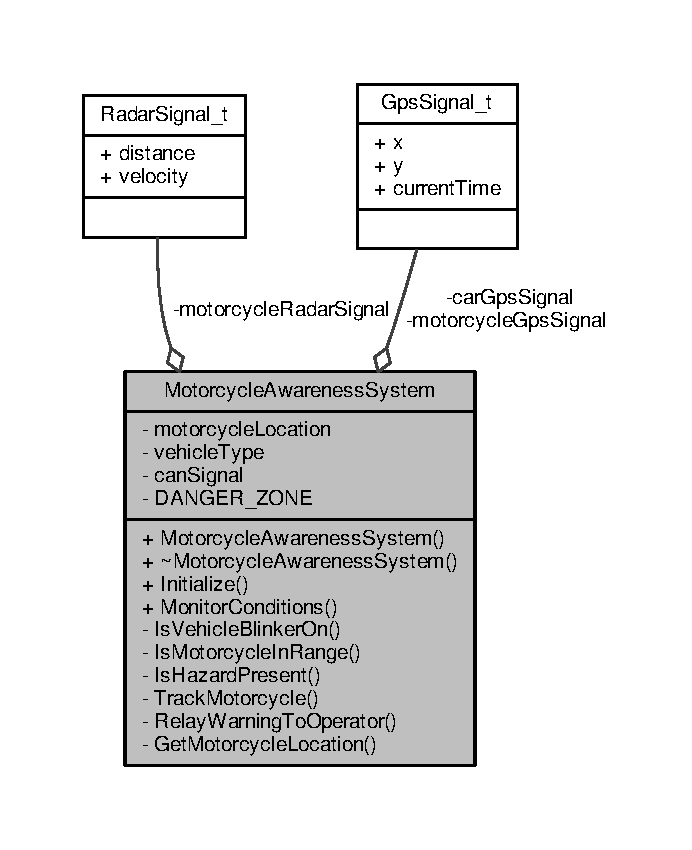
\includegraphics[width=350pt]{classMotorcycleAwarenessSystem__coll__graph}
\end{center}
\end{figure}
\subsubsection*{Public Member Functions}
\begin{DoxyCompactItemize}
\item 
\hyperlink{classMotorcycleAwarenessSystem_ab0fb3823809dc056fecc82cc72a80a55}{Motorcycle\-Awareness\-System} (\hyperlink{MotorcycleAwarenessSystemTypes_8hpp_a0c05c42b98a847f971385c81c2a81afa}{Vehicle\-Type} \hyperlink{classMotorcycleAwarenessSystem_a977b2085bfbf6a62902bf2d80160e6d2}{vehicle\-Type})
\begin{DoxyCompactList}\small\item\em Constructor. \end{DoxyCompactList}\item 
\hyperlink{classMotorcycleAwarenessSystem_a89ce16a722b3575e1415cbe9c7eedbd3}{$\sim$\-Motorcycle\-Awareness\-System} (void)
\begin{DoxyCompactList}\small\item\em Destructor. \end{DoxyCompactList}\item 
bool \hyperlink{classMotorcycleAwarenessSystem_a341f27867c8d6aa0865040279ee246a9}{Initialize} (\hyperlink{structTurnSignal__t}{Turn\-Signal\-\_\-t} $\ast$motorcycle\-Turn\-Signal, \hyperlink{structTurnSignal__t}{Turn\-Signal\-\_\-t} $\ast$car\-Turn\-Signal, \hyperlink{structRadarSignal__t}{Radar\-Signal\-\_\-t} $\ast$\hyperlink{classMotorcycleAwarenessSystem_a0744e71b9f440a86f5078c876ba7629b}{motorcycle\-Radar\-Signal}, \hyperlink{structGpsSignal__t}{Gps\-Signal\-\_\-t} $\ast$\hyperlink{classMotorcycleAwarenessSystem_ab281a3993b574923b2f379ed0477b2d4}{motorcycle\-Gps\-Signal}, \hyperlink{structGpsSignal__t}{Gps\-Signal\-\_\-t} $\ast$\hyperlink{classMotorcycleAwarenessSystem_a9a8185e00b60d0be58bfa76166063128}{car\-Gps\-Signal})
\item 
void \hyperlink{classMotorcycleAwarenessSystem_afb19e832c17d43941d9ed6c4f4435a2e}{Monitor\-Conditions} (void)
\begin{DoxyCompactList}\small\item\em Method to continuously monitor the conditions during run-\/time. \end{DoxyCompactList}\end{DoxyCompactItemize}
\subsubsection*{Private Member Functions}
\begin{DoxyCompactItemize}
\item 
bool \hyperlink{classMotorcycleAwarenessSystem_a9c3f98a014b0af39fa120f478eb5f348}{Is\-Vehicle\-Blinker\-On} (void)
\begin{DoxyCompactList}\small\item\em Method to determine whether the car's blinker is O\-N. \end{DoxyCompactList}\item 
bool \hyperlink{classMotorcycleAwarenessSystem_a239655aca9c875b1dbbad3ce155c7892}{Is\-Motorcycle\-In\-Range} (void)
\begin{DoxyCompactList}\small\item\em Method to determine whether the motorcycle is within the car's range. \end{DoxyCompactList}\item 
bool \hyperlink{classMotorcycleAwarenessSystem_a35d59c8299b0d5ef43c10306cc7f2ee1}{Is\-Hazard\-Present} (void)
\item 
void \hyperlink{classMotorcycleAwarenessSystem_a4e6eec23ec46e24ee377a3c94e15eba4}{Track\-Motorcycle} (void)
\begin{DoxyCompactList}\small\item\em Method to track the motorcycle using its G\-P\-S signal. \end{DoxyCompactList}\item 
void \hyperlink{classMotorcycleAwarenessSystem_aec5e4731c6bf0789821ba2793918e3ee}{Relay\-Warning\-To\-Operator} (void)
\begin{DoxyCompactList}\small\item\em Method to relay a warning to operator via bluetooth connectivity. \end{DoxyCompactList}\item 
\hyperlink{structMotorCycleLocation__t}{Motor\-Cycle\-Location\-\_\-t} \hyperlink{classMotorcycleAwarenessSystem_a840a5bc17d75276ecdb3a39d7aaf4109}{Get\-Motorcycle\-Location} (void)
\end{DoxyCompactItemize}
\subsubsection*{Private Attributes}
\begin{DoxyCompactItemize}
\item 
std\-::list$<$ \hyperlink{structGpsSignal__t}{Gps\-Signal\-\_\-t} $>$ \hyperlink{classMotorcycleAwarenessSystem_af6becfeb1d11b467cb80a94a8e6940ac}{motorcycle\-Location}
\begin{DoxyCompactList}\small\item\em Container used to track the motorcycle's location. \end{DoxyCompactList}\item 
\hyperlink{MotorcycleAwarenessSystemTypes_8hpp_a0c05c42b98a847f971385c81c2a81afa}{Vehicle\-Type} \hyperlink{classMotorcycleAwarenessSystem_a977b2085bfbf6a62902bf2d80160e6d2}{vehicle\-Type}
\begin{DoxyCompactList}\small\item\em The vehicle type (motorcycle or car) \end{DoxyCompactList}\item 
std\-::map$<$ \hyperlink{MotorcycleAwarenessSystemTypes_8hpp_a0c05c42b98a847f971385c81c2a81afa}{Vehicle\-Type}, \\*
\hyperlink{structTurnSignal__t}{Turn\-Signal\-\_\-t} $\ast$ $>$ \hyperlink{classMotorcycleAwarenessSystem_a43fde090639a3a58fc5bbf8bafc966f7}{turn\-Signal}
\begin{DoxyCompactList}\small\item\em Storage for the turn signals. \end{DoxyCompactList}\item 
\hyperlink{structRadarSignal__t}{Radar\-Signal\-\_\-t} $\ast$ \hyperlink{classMotorcycleAwarenessSystem_a0744e71b9f440a86f5078c876ba7629b}{motorcycle\-Radar\-Signal}
\begin{DoxyCompactList}\small\item\em Pointer to a motorcycle radar signal. \end{DoxyCompactList}\item 
\hyperlink{structGpsSignal__t}{Gps\-Signal\-\_\-t} $\ast$ \hyperlink{classMotorcycleAwarenessSystem_ab281a3993b574923b2f379ed0477b2d4}{motorcycle\-Gps\-Signal}
\begin{DoxyCompactList}\small\item\em Pointer to a motorcycle G\-P\-S signal. \end{DoxyCompactList}\item 
\hyperlink{structGpsSignal__t}{Gps\-Signal\-\_\-t} $\ast$ \hyperlink{classMotorcycleAwarenessSystem_a9a8185e00b60d0be58bfa76166063128}{car\-Gps\-Signal}
\begin{DoxyCompactList}\small\item\em Pointer to a car G\-P\-S signal. \end{DoxyCompactList}\end{DoxyCompactItemize}
\subsubsection*{Static Private Attributes}
\begin{DoxyCompactItemize}
\item 
static const unsigned int \hyperlink{classMotorcycleAwarenessSystem_a131c99d85b78020f94fe14bd397f3a6e}{S\-A\-F\-E\-T\-Y\-\_\-\-Z\-O\-N\-E} = 15\-U
\end{DoxyCompactItemize}


\subsubsection{Detailed Description}
Class declaration for the Motorcycle Awareness System (M\-A\-S) 

Definition at line \hyperlink{MotorcycleAwarenessSystem_8hpp_source_l00012}{12} of file \hyperlink{MotorcycleAwarenessSystem_8hpp_source}{Motorcycle\-Awareness\-System.\-hpp}.



\subsubsection{Constructor \& Destructor Documentation}
\hypertarget{classMotorcycleAwarenessSystem_ab0fb3823809dc056fecc82cc72a80a55}{\index{Motorcycle\-Awareness\-System@{Motorcycle\-Awareness\-System}!Motorcycle\-Awareness\-System@{Motorcycle\-Awareness\-System}}
\index{Motorcycle\-Awareness\-System@{Motorcycle\-Awareness\-System}!MotorcycleAwarenessSystem@{Motorcycle\-Awareness\-System}}
\paragraph[{Motorcycle\-Awareness\-System}]{\setlength{\rightskip}{0pt plus 5cm}Motorcycle\-Awareness\-System\-::\-Motorcycle\-Awareness\-System (
\begin{DoxyParamCaption}
\item[{{\bf Vehicle\-Type}}]{vehicle\-Type}
\end{DoxyParamCaption}
)}}\label{classMotorcycleAwarenessSystem_ab0fb3823809dc056fecc82cc72a80a55}


Constructor. 

Class definition for the Motorcycle Awareness System (M\-A\-S). This class processes various signals and interactions to realize the M\-A\-S 

Definition at line \hyperlink{MotorcycleAwarenessSystem_8cpp_source_l00013}{13} of file \hyperlink{MotorcycleAwarenessSystem_8cpp_source}{Motorcycle\-Awareness\-System.\-cpp}.


\begin{DoxyCode}
00014     :\hyperlink{classMotorcycleAwarenessSystem_a977b2085bfbf6a62902bf2d80160e6d2}{vehicleType}( \hyperlink{classMotorcycleAwarenessSystem_a977b2085bfbf6a62902bf2d80160e6d2}{vehicleType} )
00015 \{
00016     \textcolor{comment}{// Do nothing}
00017 \}
\end{DoxyCode}
\hypertarget{classMotorcycleAwarenessSystem_a89ce16a722b3575e1415cbe9c7eedbd3}{\index{Motorcycle\-Awareness\-System@{Motorcycle\-Awareness\-System}!$\sim$\-Motorcycle\-Awareness\-System@{$\sim$\-Motorcycle\-Awareness\-System}}
\index{$\sim$\-Motorcycle\-Awareness\-System@{$\sim$\-Motorcycle\-Awareness\-System}!MotorcycleAwarenessSystem@{Motorcycle\-Awareness\-System}}
\paragraph[{$\sim$\-Motorcycle\-Awareness\-System}]{\setlength{\rightskip}{0pt plus 5cm}Motorcycle\-Awareness\-System\-::$\sim$\-Motorcycle\-Awareness\-System (
\begin{DoxyParamCaption}
\item[{void}]{}
\end{DoxyParamCaption}
)}}\label{classMotorcycleAwarenessSystem_a89ce16a722b3575e1415cbe9c7eedbd3}


Destructor. 



Definition at line \hyperlink{MotorcycleAwarenessSystem_8cpp_source_l00020}{20} of file \hyperlink{MotorcycleAwarenessSystem_8cpp_source}{Motorcycle\-Awareness\-System.\-cpp}.


\begin{DoxyCode}
00021 \{
00022     \textcolor{comment}{// Do nothing}
00023 \}
\end{DoxyCode}


\subsubsection{Member Function Documentation}
\hypertarget{classMotorcycleAwarenessSystem_a840a5bc17d75276ecdb3a39d7aaf4109}{\index{Motorcycle\-Awareness\-System@{Motorcycle\-Awareness\-System}!Get\-Motorcycle\-Location@{Get\-Motorcycle\-Location}}
\index{Get\-Motorcycle\-Location@{Get\-Motorcycle\-Location}!MotorcycleAwarenessSystem@{Motorcycle\-Awareness\-System}}
\paragraph[{Get\-Motorcycle\-Location}]{\setlength{\rightskip}{0pt plus 5cm}{\bf Motor\-Cycle\-Location\-\_\-t} Motorcycle\-Awareness\-System\-::\-Get\-Motorcycle\-Location (
\begin{DoxyParamCaption}
\item[{void}]{}
\end{DoxyParamCaption}
)\hspace{0.3cm}{\ttfamily [private]}}}\label{classMotorcycleAwarenessSystem_a840a5bc17d75276ecdb3a39d7aaf4109}
\begin{DoxyRefDesc}{Todo}
\item[\hyperlink{todo__todo000003}{Todo}]Acquire the data packet from the motorcycle \end{DoxyRefDesc}


Definition at line \hyperlink{MotorcycleAwarenessSystem_8cpp_source_l00163}{163} of file \hyperlink{MotorcycleAwarenessSystem_8cpp_source}{Motorcycle\-Awareness\-System.\-cpp}.


\begin{DoxyCode}
00164 \{
00165     \textcolor{comment}{// Dummy motorcycle location from V2V communication}
00166     \hyperlink{structMotorCycleLocation__t}{MotorCycleLocation\_t} motorCycleLocation;
00168 
00169     \textcolor{keywordflow}{return} motorCycleLocation;
00170 \}
\end{DoxyCode}


Here is the caller graph for this function\-:\nopagebreak
\begin{figure}[H]
\begin{center}
\leavevmode
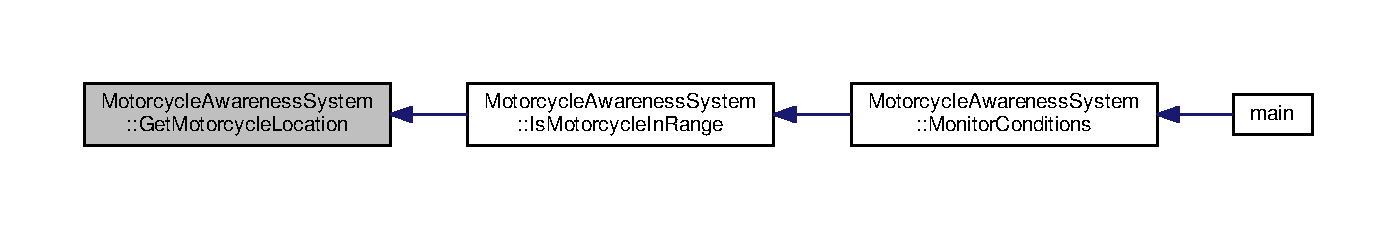
\includegraphics[width=350pt]{classMotorcycleAwarenessSystem_a840a5bc17d75276ecdb3a39d7aaf4109_icgraph}
\end{center}
\end{figure}


\hypertarget{classMotorcycleAwarenessSystem_a341f27867c8d6aa0865040279ee246a9}{\index{Motorcycle\-Awareness\-System@{Motorcycle\-Awareness\-System}!Initialize@{Initialize}}
\index{Initialize@{Initialize}!MotorcycleAwarenessSystem@{Motorcycle\-Awareness\-System}}
\paragraph[{Initialize}]{\setlength{\rightskip}{0pt plus 5cm}bool Motorcycle\-Awareness\-System\-::\-Initialize (
\begin{DoxyParamCaption}
\item[{{\bf Turn\-Signal\-\_\-t} $\ast$}]{motorcycle\-Turn\-Signal, }
\item[{{\bf Turn\-Signal\-\_\-t} $\ast$}]{car\-Turn\-Signal, }
\item[{{\bf Radar\-Signal\-\_\-t} $\ast$}]{motorcycle\-Radar\-Signal, }
\item[{{\bf Gps\-Signal\-\_\-t} $\ast$}]{motorcycle\-Gps\-Signal, }
\item[{{\bf Gps\-Signal\-\_\-t} $\ast$}]{car\-Gps\-Signal}
\end{DoxyParamCaption}
)}}\label{classMotorcycleAwarenessSystem_a341f27867c8d6aa0865040279ee246a9}
Method to initialize the M\-A\-S system


\begin{DoxyParams}[1]{Parameters}
\mbox{\tt in}  & {\em motorcycle\-Turn\-Signal} & Motorcycle turn signal \\
\hline
\mbox{\tt in}  & {\em car\-Turn\-Signal} & Car turn signal \\
\hline
\mbox{\tt in}  & {\em motorcycle\-Radar\-Signal} & Motorcycle radar signal \\
\hline
\mbox{\tt in}  & {\em motorcycle\-Gps\-Signal} & Motorcycle G\-P\-S signal \\
\hline
\mbox{\tt in}  & {\em car\-Gps\-Signal} & Car G\-P\-S signal\\
\hline
\end{DoxyParams}
\begin{DoxyReturn}{Returns}
Pass fail status of the initialization
\end{DoxyReturn}

\begin{DoxyRetVals}{Return values}
{\em true} & \\
\hline
{\em false} & \\
\hline
\end{DoxyRetVals}


Definition at line \hyperlink{MotorcycleAwarenessSystem_8cpp_source_l00038}{38} of file \hyperlink{MotorcycleAwarenessSystem_8cpp_source}{Motorcycle\-Awareness\-System.\-cpp}.


\begin{DoxyCode}
00041 \{
00042     \textcolor{comment}{// Initialize the initialization state}
00043     \textcolor{keywordtype}{bool} isSuccess = \textcolor{keyword}{false};
00044 
00045     \textcolor{keywordflow}{if} ( motorcycleTurnSignal != (\hyperlink{structTurnSignal__t}{TurnSignal\_t}*)NULL &&
00046          carTurnSignal != (\hyperlink{structTurnSignal__t}{TurnSignal\_t}*)NULL &&
00047          motorcycleRadarSignal != (\hyperlink{structRadarSignal__t}{RadarSignal\_t}*)NULL &&
00048          motorcycleGpsSignal != (\hyperlink{structGpsSignal__t}{GpsSignal\_t}*)NULL &&
00049          carGpsSignal != (\hyperlink{structGpsSignal__t}{GpsSignal\_t}*)NULL )
00050     \{
00051         \textcolor{comment}{// Initialize the motorcycle radar signal}
00052         this->motorcycleRadarSignal = \hyperlink{classMotorcycleAwarenessSystem_a0744e71b9f440a86f5078c876ba7629b}{motorcycleRadarSignal};
00053 
00054         \textcolor{comment}{// Initialize the turn signal map}
00055         \hyperlink{classMotorcycleAwarenessSystem_a43fde090639a3a58fc5bbf8bafc966f7}{turnSignal}[\hyperlink{MotorcycleAwarenessSystemTypes_8hpp_a0c05c42b98a847f971385c81c2a81afaa39b983b1f7acfc4e7c900d77b0fded6a}{MOTORCYCLE}] = motorcycleTurnSignal;
00056         \hyperlink{classMotorcycleAwarenessSystem_a43fde090639a3a58fc5bbf8bafc966f7}{turnSignal}[\hyperlink{MotorcycleAwarenessSystemTypes_8hpp_a0c05c42b98a847f971385c81c2a81afaa5fc54ebcb1dd4bf1e1b93cbc77b57b40}{CAR}] = carTurnSignal;
00057 
00058         \textcolor{comment}{// Initialize the GPS signals}
00059         this->motorcycleGpsSignal = \hyperlink{classMotorcycleAwarenessSystem_ab281a3993b574923b2f379ed0477b2d4}{motorcycleGpsSignal};
00060         this->carGpsSignal = \hyperlink{classMotorcycleAwarenessSystem_a9a8185e00b60d0be58bfa76166063128}{carGpsSignal};
00061 
00062         isSuccess = \textcolor{keyword}{true};
00063     \}
00064 
00065     \textcolor{keywordflow}{return} isSuccess;
00066 \}
\end{DoxyCode}


Here is the caller graph for this function\-:\nopagebreak
\begin{figure}[H]
\begin{center}
\leavevmode
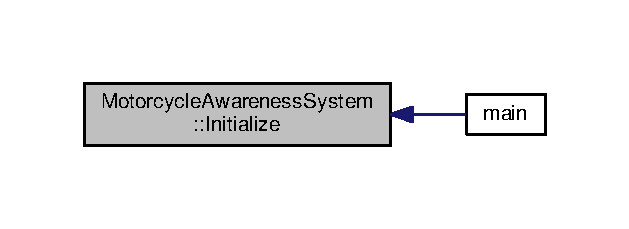
\includegraphics[width=302pt]{classMotorcycleAwarenessSystem_a341f27867c8d6aa0865040279ee246a9_icgraph}
\end{center}
\end{figure}


\hypertarget{classMotorcycleAwarenessSystem_a35d59c8299b0d5ef43c10306cc7f2ee1}{\index{Motorcycle\-Awareness\-System@{Motorcycle\-Awareness\-System}!Is\-Hazard\-Present@{Is\-Hazard\-Present}}
\index{Is\-Hazard\-Present@{Is\-Hazard\-Present}!MotorcycleAwarenessSystem@{Motorcycle\-Awareness\-System}}
\paragraph[{Is\-Hazard\-Present}]{\setlength{\rightskip}{0pt plus 5cm}bool Motorcycle\-Awareness\-System\-::\-Is\-Hazard\-Present (
\begin{DoxyParamCaption}
\item[{void}]{}
\end{DoxyParamCaption}
)\hspace{0.3cm}{\ttfamily [private]}}}\label{classMotorcycleAwarenessSystem_a35d59c8299b0d5ef43c10306cc7f2ee1}
Method to determine whether a hazard is within the motorcycle's safety zone. An object within the safety zone is of potential danger to the motorcycle rider. 

Definition at line \hyperlink{MotorcycleAwarenessSystem_8cpp_source_l00131}{131} of file \hyperlink{MotorcycleAwarenessSystem_8cpp_source}{Motorcycle\-Awareness\-System.\-cpp}.


\begin{DoxyCode}
00132 \{
00133     \textcolor{keywordtype}{bool} isHazardPresent = \textcolor{keyword}{false};
00134 
00135     \textcolor{keywordflow}{if} ( abs( this->\hyperlink{classMotorcycleAwarenessSystem_a0744e71b9f440a86f5078c876ba7629b}{motorcycleRadarSignal}->\hyperlink{structRadarSignal__t_a96938fbfb77f208743a36d3f8b37cccb}{objectDistance} ) <= 
      \hyperlink{classMotorcycleAwarenessSystem_a131c99d85b78020f94fe14bd397f3a6e}{SAFETY\_ZONE} )
00136     \{
00137         isHazardPresent = \textcolor{keyword}{true};
00138     \}
00139 
00140     \textcolor{keywordflow}{return} isHazardPresent;
00141 \}
\end{DoxyCode}


Here is the caller graph for this function\-:\nopagebreak
\begin{figure}[H]
\begin{center}
\leavevmode
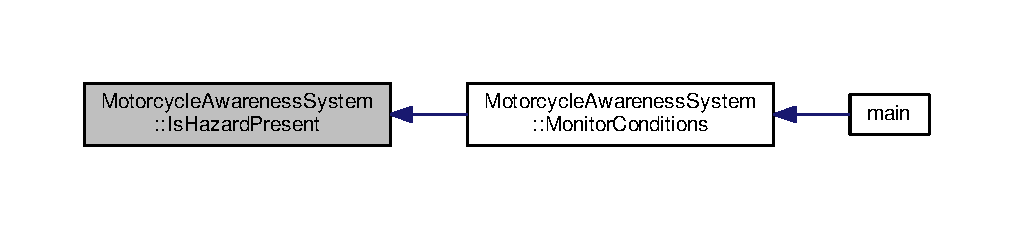
\includegraphics[width=350pt]{classMotorcycleAwarenessSystem_a35d59c8299b0d5ef43c10306cc7f2ee1_icgraph}
\end{center}
\end{figure}


\hypertarget{classMotorcycleAwarenessSystem_a239655aca9c875b1dbbad3ce155c7892}{\index{Motorcycle\-Awareness\-System@{Motorcycle\-Awareness\-System}!Is\-Motorcycle\-In\-Range@{Is\-Motorcycle\-In\-Range}}
\index{Is\-Motorcycle\-In\-Range@{Is\-Motorcycle\-In\-Range}!MotorcycleAwarenessSystem@{Motorcycle\-Awareness\-System}}
\paragraph[{Is\-Motorcycle\-In\-Range}]{\setlength{\rightskip}{0pt plus 5cm}bool Motorcycle\-Awareness\-System\-::\-Is\-Motorcycle\-In\-Range (
\begin{DoxyParamCaption}
\item[{void}]{}
\end{DoxyParamCaption}
)\hspace{0.3cm}{\ttfamily [private]}}}\label{classMotorcycleAwarenessSystem_a239655aca9c875b1dbbad3ce155c7892}


Method to determine whether the motorcycle is within the car's range. 

\begin{DoxyRefDesc}{Todo}
\item[\hyperlink{todo__todo000001}{Todo}]Process the data packet and determine threat \end{DoxyRefDesc}


Definition at line \hyperlink{MotorcycleAwarenessSystem_8cpp_source_l00109}{109} of file \hyperlink{MotorcycleAwarenessSystem_8cpp_source}{Motorcycle\-Awareness\-System.\-cpp}.


\begin{DoxyCode}
00110 \{
00111     \textcolor{keywordtype}{bool} isInRange = \textcolor{keyword}{false};
00112 
00113     \textcolor{comment}{// Determine where the motorcycle is relative to the car using the GPS signals}
00114     \textcolor{keywordflow}{if} ( abs( (this->\hyperlink{classMotorcycleAwarenessSystem_a9a8185e00b60d0be58bfa76166063128}{carGpsSignal}->\hyperlink{structGpsSignal__t_a6f7bd3c500b55923ab335ada4b6b26eb}{x}) - (this->motorcycleGpsSignal->x) ) <= 
      \hyperlink{classMotorcycleAwarenessSystem_a131c99d85b78020f94fe14bd397f3a6e}{SAFETY\_ZONE} &&
00115          abs( (this->\hyperlink{classMotorcycleAwarenessSystem_a9a8185e00b60d0be58bfa76166063128}{carGpsSignal}->\hyperlink{structGpsSignal__t_ab9e083be189fc842ed7aa4fdc978e94e}{y}) - (this->motorcycleGpsSignal->y) ) <= 
      \hyperlink{classMotorcycleAwarenessSystem_a131c99d85b78020f94fe14bd397f3a6e}{SAFETY\_ZONE} )
00116     \{
00117         isInRange = \textcolor{keyword}{true};
00118     \}
00119     \textcolor{keywordflow}{else}
00120     \{
00121         \textcolor{comment}{// Analyze the V2V data for a threat}
00122         \hyperlink{structMotorCycleLocation__t}{MotorCycleLocation\_t} motorCycleLocation = 
      \hyperlink{classMotorcycleAwarenessSystem_a840a5bc17d75276ecdb3a39d7aaf4109}{GetMotorcycleLocation}();
00124     \}
00125 
00126     \textcolor{keywordflow}{return} isInRange;
00127 \}
\end{DoxyCode}


Here is the call graph for this function\-:\nopagebreak
\begin{figure}[H]
\begin{center}
\leavevmode
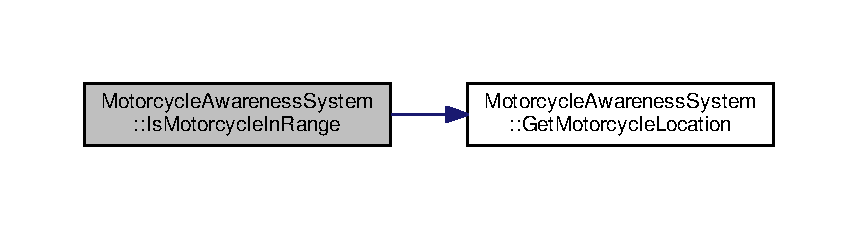
\includegraphics[width=350pt]{classMotorcycleAwarenessSystem_a239655aca9c875b1dbbad3ce155c7892_cgraph}
\end{center}
\end{figure}




Here is the caller graph for this function\-:\nopagebreak
\begin{figure}[H]
\begin{center}
\leavevmode
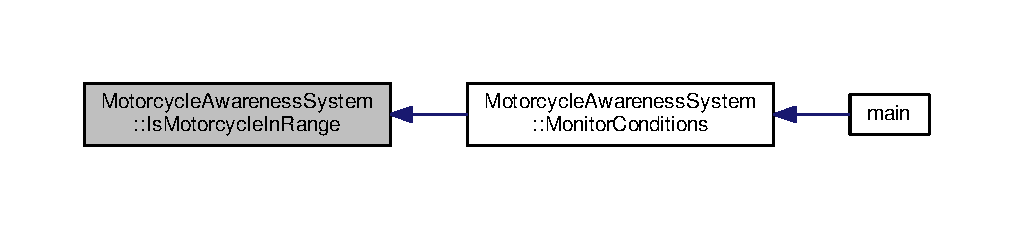
\includegraphics[width=350pt]{classMotorcycleAwarenessSystem_a239655aca9c875b1dbbad3ce155c7892_icgraph}
\end{center}
\end{figure}


\hypertarget{classMotorcycleAwarenessSystem_a9c3f98a014b0af39fa120f478eb5f348}{\index{Motorcycle\-Awareness\-System@{Motorcycle\-Awareness\-System}!Is\-Vehicle\-Blinker\-On@{Is\-Vehicle\-Blinker\-On}}
\index{Is\-Vehicle\-Blinker\-On@{Is\-Vehicle\-Blinker\-On}!MotorcycleAwarenessSystem@{Motorcycle\-Awareness\-System}}
\paragraph[{Is\-Vehicle\-Blinker\-On}]{\setlength{\rightskip}{0pt plus 5cm}bool Motorcycle\-Awareness\-System\-::\-Is\-Vehicle\-Blinker\-On (
\begin{DoxyParamCaption}
\item[{void}]{}
\end{DoxyParamCaption}
)\hspace{0.3cm}{\ttfamily [private]}}}\label{classMotorcycleAwarenessSystem_a9c3f98a014b0af39fa120f478eb5f348}


Method to determine whether the car's blinker is O\-N. 



Definition at line \hyperlink{MotorcycleAwarenessSystem_8cpp_source_l00095}{95} of file \hyperlink{MotorcycleAwarenessSystem_8cpp_source}{Motorcycle\-Awareness\-System.\-cpp}.


\begin{DoxyCode}
00096 \{
00097     \textcolor{keywordtype}{bool} isBlinkerOn = \textcolor{keyword}{false};
00098 
00099     \textcolor{keywordflow}{if} ( this->\hyperlink{classMotorcycleAwarenessSystem_a43fde090639a3a58fc5bbf8bafc966f7}{turnSignal}[\hyperlink{classMotorcycleAwarenessSystem_a977b2085bfbf6a62902bf2d80160e6d2}{vehicleType}]->isRightBlinkerOn ||
00100          this->\hyperlink{classMotorcycleAwarenessSystem_a43fde090639a3a58fc5bbf8bafc966f7}{turnSignal}[\hyperlink{classMotorcycleAwarenessSystem_a977b2085bfbf6a62902bf2d80160e6d2}{vehicleType}]->isLeftBlinkerOn )
00101     \{
00102         isBlinkerOn = \textcolor{keyword}{true};
00103     \}
00104 
00105     \textcolor{keywordflow}{return} isBlinkerOn;
00106 \}
\end{DoxyCode}


Here is the caller graph for this function\-:\nopagebreak
\begin{figure}[H]
\begin{center}
\leavevmode
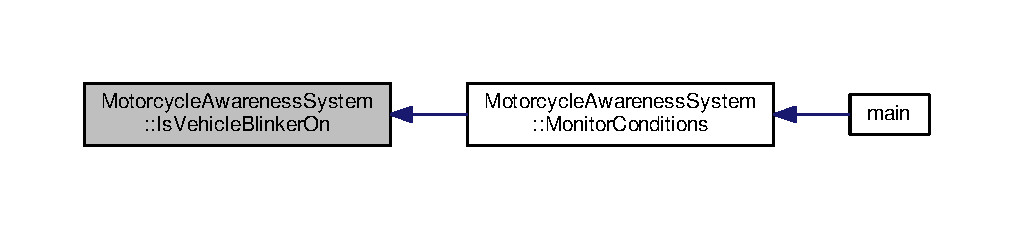
\includegraphics[width=350pt]{classMotorcycleAwarenessSystem_a9c3f98a014b0af39fa120f478eb5f348_icgraph}
\end{center}
\end{figure}


\hypertarget{classMotorcycleAwarenessSystem_afb19e832c17d43941d9ed6c4f4435a2e}{\index{Motorcycle\-Awareness\-System@{Motorcycle\-Awareness\-System}!Monitor\-Conditions@{Monitor\-Conditions}}
\index{Monitor\-Conditions@{Monitor\-Conditions}!MotorcycleAwarenessSystem@{Motorcycle\-Awareness\-System}}
\paragraph[{Monitor\-Conditions}]{\setlength{\rightskip}{0pt plus 5cm}void Motorcycle\-Awareness\-System\-::\-Monitor\-Conditions (
\begin{DoxyParamCaption}
\item[{void}]{}
\end{DoxyParamCaption}
)}}\label{classMotorcycleAwarenessSystem_afb19e832c17d43941d9ed6c4f4435a2e}


Method to continuously monitor the conditions during run-\/time. 



Definition at line \hyperlink{MotorcycleAwarenessSystem_8cpp_source_l00069}{69} of file \hyperlink{MotorcycleAwarenessSystem_8cpp_source}{Motorcycle\-Awareness\-System.\-cpp}.


\begin{DoxyCode}
00070 \{
00071     \textcolor{keywordflow}{if} ( \hyperlink{MotorcycleAwarenessSystemTypes_8hpp_a0c05c42b98a847f971385c81c2a81afaa39b983b1f7acfc4e7c900d77b0fded6a}{MOTORCYCLE} == \hyperlink{classMotorcycleAwarenessSystem_a977b2085bfbf6a62902bf2d80160e6d2}{vehicleType} )
00072     \{
00073         \textcolor{comment}{// Track the motorcycle}
00074         \hyperlink{classMotorcycleAwarenessSystem_a4e6eec23ec46e24ee377a3c94e15eba4}{TrackMotorcycle}();
00075         \textcolor{comment}{// Check for hazards}
00076         \textcolor{keywordflow}{if} ( \hyperlink{classMotorcycleAwarenessSystem_a35d59c8299b0d5ef43c10306cc7f2ee1}{IsHazardPresent}() == \textcolor{keyword}{true} )
00077         \{
00078             \textcolor{comment}{// Warn the motorcycle operator}
00079             \hyperlink{classMotorcycleAwarenessSystem_aec5e4731c6bf0789821ba2793918e3ee}{RelayWarningToOperator}();
00080         \}
00081     \}
00082     \textcolor{comment}{// vehicleType == CAR}
00083     \textcolor{keywordflow}{else}
00084     \{
00085         \textcolor{comment}{// Check for hazards}
00086         \textcolor{keywordflow}{if} ( (\hyperlink{classMotorcycleAwarenessSystem_a9c3f98a014b0af39fa120f478eb5f348}{IsVehicleBlinkerOn}() == \textcolor{keyword}{true}) && (
      \hyperlink{classMotorcycleAwarenessSystem_a239655aca9c875b1dbbad3ce155c7892}{IsMotorcycleInRange}() == \textcolor{keyword}{true}) )
00087         \{
00088             \textcolor{comment}{// Relay message to the car driver}
00089             \hyperlink{classMotorcycleAwarenessSystem_aec5e4731c6bf0789821ba2793918e3ee}{RelayWarningToOperator}();
00090         \}
00091     \}
00092 \}
\end{DoxyCode}


Here is the call graph for this function\-:\nopagebreak
\begin{figure}[H]
\begin{center}
\leavevmode
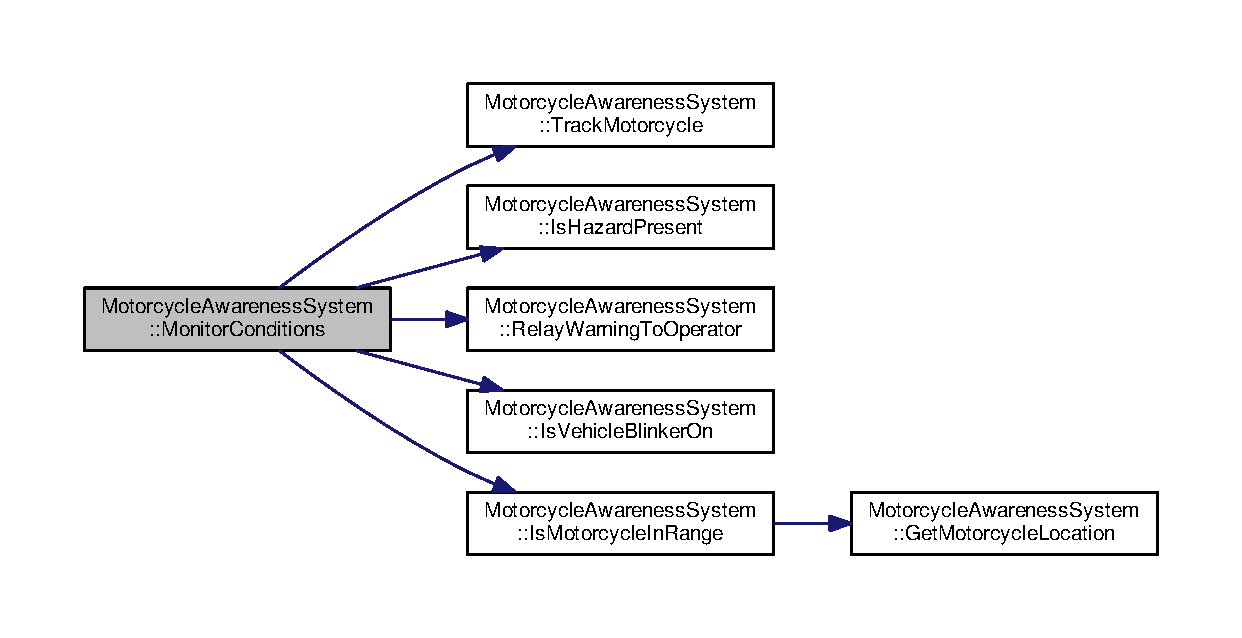
\includegraphics[width=350pt]{classMotorcycleAwarenessSystem_afb19e832c17d43941d9ed6c4f4435a2e_cgraph}
\end{center}
\end{figure}




Here is the caller graph for this function\-:\nopagebreak
\begin{figure}[H]
\begin{center}
\leavevmode
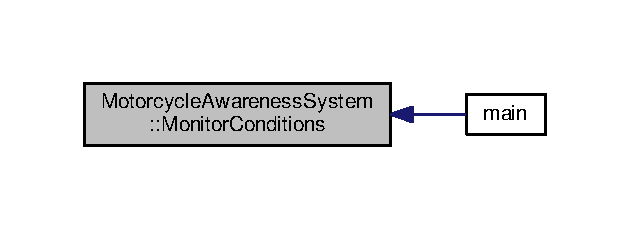
\includegraphics[width=302pt]{classMotorcycleAwarenessSystem_afb19e832c17d43941d9ed6c4f4435a2e_icgraph}
\end{center}
\end{figure}


\hypertarget{classMotorcycleAwarenessSystem_aec5e4731c6bf0789821ba2793918e3ee}{\index{Motorcycle\-Awareness\-System@{Motorcycle\-Awareness\-System}!Relay\-Warning\-To\-Operator@{Relay\-Warning\-To\-Operator}}
\index{Relay\-Warning\-To\-Operator@{Relay\-Warning\-To\-Operator}!MotorcycleAwarenessSystem@{Motorcycle\-Awareness\-System}}
\paragraph[{Relay\-Warning\-To\-Operator}]{\setlength{\rightskip}{0pt plus 5cm}void Motorcycle\-Awareness\-System\-::\-Relay\-Warning\-To\-Operator (
\begin{DoxyParamCaption}
\item[{void}]{}
\end{DoxyParamCaption}
)\hspace{0.3cm}{\ttfamily [private]}}}\label{classMotorcycleAwarenessSystem_aec5e4731c6bf0789821ba2793918e3ee}


Method to relay a warning to operator via bluetooth connectivity. 

\begin{DoxyRefDesc}{Todo}
\item[\hyperlink{todo__todo000002}{Todo}]Transmit the bluetooth message to the operator \end{DoxyRefDesc}


Definition at line \hyperlink{MotorcycleAwarenessSystem_8cpp_source_l00151}{151} of file \hyperlink{MotorcycleAwarenessSystem_8cpp_source}{Motorcycle\-Awareness\-System.\-cpp}.


\begin{DoxyCode}
00152 \{
00153     \textcolor{comment}{// Assemble the message to be sent}
00154     \hyperlink{structBlueToothMessage__t}{BlueToothMessage\_t} blueToothMessage;
00155     blueToothMessage.\hyperlink{structBlueToothMessage__t_a2dd315aa1cba1d2d3045e26b9f171e61}{isHazardPresent} = \textcolor{keyword}{true};
00156     \textcolor{comment}{// Dummy message}
00157     blueToothMessage.\hyperlink{structBlueToothMessage__t_ab872789a32f068dae8bcf77122256b78}{dataBuffer}[0] = 0x2015;
00158 
00160 \}
\end{DoxyCode}


Here is the caller graph for this function\-:\nopagebreak
\begin{figure}[H]
\begin{center}
\leavevmode
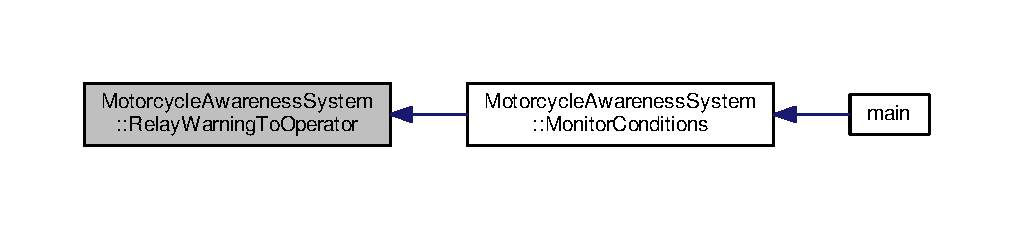
\includegraphics[width=350pt]{classMotorcycleAwarenessSystem_aec5e4731c6bf0789821ba2793918e3ee_icgraph}
\end{center}
\end{figure}


\hypertarget{classMotorcycleAwarenessSystem_a4e6eec23ec46e24ee377a3c94e15eba4}{\index{Motorcycle\-Awareness\-System@{Motorcycle\-Awareness\-System}!Track\-Motorcycle@{Track\-Motorcycle}}
\index{Track\-Motorcycle@{Track\-Motorcycle}!MotorcycleAwarenessSystem@{Motorcycle\-Awareness\-System}}
\paragraph[{Track\-Motorcycle}]{\setlength{\rightskip}{0pt plus 5cm}void Motorcycle\-Awareness\-System\-::\-Track\-Motorcycle (
\begin{DoxyParamCaption}
\item[{void}]{}
\end{DoxyParamCaption}
)\hspace{0.3cm}{\ttfamily [private]}}}\label{classMotorcycleAwarenessSystem_a4e6eec23ec46e24ee377a3c94e15eba4}


Method to track the motorcycle using its G\-P\-S signal. 



Definition at line \hyperlink{MotorcycleAwarenessSystem_8cpp_source_l00144}{144} of file \hyperlink{MotorcycleAwarenessSystem_8cpp_source}{Motorcycle\-Awareness\-System.\-cpp}.


\begin{DoxyCode}
00145 \{
00146     \textcolor{comment}{// Push the motorcycle's GPS location onto the list}
00147     \hyperlink{classMotorcycleAwarenessSystem_af6becfeb1d11b467cb80a94a8e6940ac}{motorcycleLocation}.push\_front( *\hyperlink{classMotorcycleAwarenessSystem_ab281a3993b574923b2f379ed0477b2d4}{motorcycleGpsSignal} );
00148 \}
\end{DoxyCode}


Here is the caller graph for this function\-:\nopagebreak
\begin{figure}[H]
\begin{center}
\leavevmode
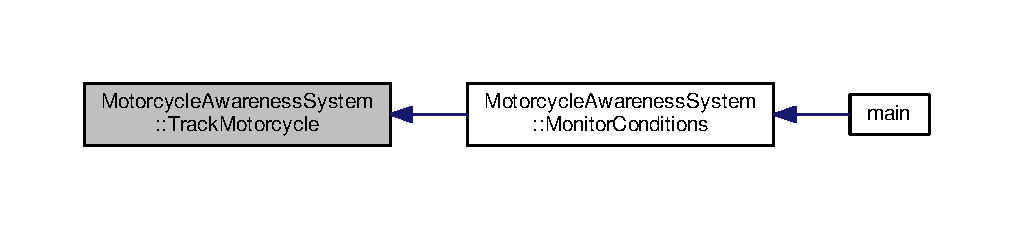
\includegraphics[width=350pt]{classMotorcycleAwarenessSystem_a4e6eec23ec46e24ee377a3c94e15eba4_icgraph}
\end{center}
\end{figure}




\subsubsection{Member Data Documentation}
\hypertarget{classMotorcycleAwarenessSystem_a9a8185e00b60d0be58bfa76166063128}{\index{Motorcycle\-Awareness\-System@{Motorcycle\-Awareness\-System}!car\-Gps\-Signal@{car\-Gps\-Signal}}
\index{car\-Gps\-Signal@{car\-Gps\-Signal}!MotorcycleAwarenessSystem@{Motorcycle\-Awareness\-System}}
\paragraph[{car\-Gps\-Signal}]{\setlength{\rightskip}{0pt plus 5cm}{\bf Gps\-Signal\-\_\-t}$\ast$ Motorcycle\-Awareness\-System\-::car\-Gps\-Signal\hspace{0.3cm}{\ttfamily [private]}}}\label{classMotorcycleAwarenessSystem_a9a8185e00b60d0be58bfa76166063128}


Pointer to a car G\-P\-S signal. 



Definition at line \hyperlink{MotorcycleAwarenessSystem_8hpp_source_l00030}{30} of file \hyperlink{MotorcycleAwarenessSystem_8hpp_source}{Motorcycle\-Awareness\-System.\-hpp}.

\hypertarget{classMotorcycleAwarenessSystem_ab281a3993b574923b2f379ed0477b2d4}{\index{Motorcycle\-Awareness\-System@{Motorcycle\-Awareness\-System}!motorcycle\-Gps\-Signal@{motorcycle\-Gps\-Signal}}
\index{motorcycle\-Gps\-Signal@{motorcycle\-Gps\-Signal}!MotorcycleAwarenessSystem@{Motorcycle\-Awareness\-System}}
\paragraph[{motorcycle\-Gps\-Signal}]{\setlength{\rightskip}{0pt plus 5cm}{\bf Gps\-Signal\-\_\-t}$\ast$ Motorcycle\-Awareness\-System\-::motorcycle\-Gps\-Signal\hspace{0.3cm}{\ttfamily [private]}}}\label{classMotorcycleAwarenessSystem_ab281a3993b574923b2f379ed0477b2d4}


Pointer to a motorcycle G\-P\-S signal. 



Definition at line \hyperlink{MotorcycleAwarenessSystem_8hpp_source_l00029}{29} of file \hyperlink{MotorcycleAwarenessSystem_8hpp_source}{Motorcycle\-Awareness\-System.\-hpp}.

\hypertarget{classMotorcycleAwarenessSystem_af6becfeb1d11b467cb80a94a8e6940ac}{\index{Motorcycle\-Awareness\-System@{Motorcycle\-Awareness\-System}!motorcycle\-Location@{motorcycle\-Location}}
\index{motorcycle\-Location@{motorcycle\-Location}!MotorcycleAwarenessSystem@{Motorcycle\-Awareness\-System}}
\paragraph[{motorcycle\-Location}]{\setlength{\rightskip}{0pt plus 5cm}std\-::list$<${\bf Gps\-Signal\-\_\-t}$>$ Motorcycle\-Awareness\-System\-::motorcycle\-Location\hspace{0.3cm}{\ttfamily [private]}}}\label{classMotorcycleAwarenessSystem_af6becfeb1d11b467cb80a94a8e6940ac}


Container used to track the motorcycle's location. 



Definition at line \hyperlink{MotorcycleAwarenessSystem_8hpp_source_l00023}{23} of file \hyperlink{MotorcycleAwarenessSystem_8hpp_source}{Motorcycle\-Awareness\-System.\-hpp}.

\hypertarget{classMotorcycleAwarenessSystem_a0744e71b9f440a86f5078c876ba7629b}{\index{Motorcycle\-Awareness\-System@{Motorcycle\-Awareness\-System}!motorcycle\-Radar\-Signal@{motorcycle\-Radar\-Signal}}
\index{motorcycle\-Radar\-Signal@{motorcycle\-Radar\-Signal}!MotorcycleAwarenessSystem@{Motorcycle\-Awareness\-System}}
\paragraph[{motorcycle\-Radar\-Signal}]{\setlength{\rightskip}{0pt plus 5cm}{\bf Radar\-Signal\-\_\-t}$\ast$ Motorcycle\-Awareness\-System\-::motorcycle\-Radar\-Signal\hspace{0.3cm}{\ttfamily [private]}}}\label{classMotorcycleAwarenessSystem_a0744e71b9f440a86f5078c876ba7629b}


Pointer to a motorcycle radar signal. 



Definition at line \hyperlink{MotorcycleAwarenessSystem_8hpp_source_l00028}{28} of file \hyperlink{MotorcycleAwarenessSystem_8hpp_source}{Motorcycle\-Awareness\-System.\-hpp}.

\hypertarget{classMotorcycleAwarenessSystem_a131c99d85b78020f94fe14bd397f3a6e}{\index{Motorcycle\-Awareness\-System@{Motorcycle\-Awareness\-System}!S\-A\-F\-E\-T\-Y\-\_\-\-Z\-O\-N\-E@{S\-A\-F\-E\-T\-Y\-\_\-\-Z\-O\-N\-E}}
\index{S\-A\-F\-E\-T\-Y\-\_\-\-Z\-O\-N\-E@{S\-A\-F\-E\-T\-Y\-\_\-\-Z\-O\-N\-E}!MotorcycleAwarenessSystem@{Motorcycle\-Awareness\-System}}
\paragraph[{S\-A\-F\-E\-T\-Y\-\_\-\-Z\-O\-N\-E}]{\setlength{\rightskip}{0pt plus 5cm}const unsigned int Motorcycle\-Awareness\-System\-::\-S\-A\-F\-E\-T\-Y\-\_\-\-Z\-O\-N\-E = 15\-U\hspace{0.3cm}{\ttfamily [static]}, {\ttfamily [private]}}}\label{classMotorcycleAwarenessSystem_a131c99d85b78020f94fe14bd397f3a6e}
Distance from the radar sensor in feet in which a detected object becomes a potential danger 

Definition at line \hyperlink{MotorcycleAwarenessSystem_8hpp_source_l00024}{24} of file \hyperlink{MotorcycleAwarenessSystem_8hpp_source}{Motorcycle\-Awareness\-System.\-hpp}.

\hypertarget{classMotorcycleAwarenessSystem_a43fde090639a3a58fc5bbf8bafc966f7}{\index{Motorcycle\-Awareness\-System@{Motorcycle\-Awareness\-System}!turn\-Signal@{turn\-Signal}}
\index{turn\-Signal@{turn\-Signal}!MotorcycleAwarenessSystem@{Motorcycle\-Awareness\-System}}
\paragraph[{turn\-Signal}]{\setlength{\rightskip}{0pt plus 5cm}std\-::map$<${\bf Vehicle\-Type}, {\bf Turn\-Signal\-\_\-t}$\ast$$>$ Motorcycle\-Awareness\-System\-::turn\-Signal\hspace{0.3cm}{\ttfamily [private]}}}\label{classMotorcycleAwarenessSystem_a43fde090639a3a58fc5bbf8bafc966f7}


Storage for the turn signals. 



Definition at line \hyperlink{MotorcycleAwarenessSystem_8hpp_source_l00027}{27} of file \hyperlink{MotorcycleAwarenessSystem_8hpp_source}{Motorcycle\-Awareness\-System.\-hpp}.

\hypertarget{classMotorcycleAwarenessSystem_a977b2085bfbf6a62902bf2d80160e6d2}{\index{Motorcycle\-Awareness\-System@{Motorcycle\-Awareness\-System}!vehicle\-Type@{vehicle\-Type}}
\index{vehicle\-Type@{vehicle\-Type}!MotorcycleAwarenessSystem@{Motorcycle\-Awareness\-System}}
\paragraph[{vehicle\-Type}]{\setlength{\rightskip}{0pt plus 5cm}{\bf Vehicle\-Type} Motorcycle\-Awareness\-System\-::vehicle\-Type\hspace{0.3cm}{\ttfamily [private]}}}\label{classMotorcycleAwarenessSystem_a977b2085bfbf6a62902bf2d80160e6d2}


The vehicle type (motorcycle or car) 



Definition at line \hyperlink{MotorcycleAwarenessSystem_8hpp_source_l00026}{26} of file \hyperlink{MotorcycleAwarenessSystem_8hpp_source}{Motorcycle\-Awareness\-System.\-hpp}.



The documentation for this class was generated from the following files\-:\begin{DoxyCompactItemize}
\item 
\hyperlink{MotorcycleAwarenessSystem_8hpp}{Motorcycle\-Awareness\-System.\-hpp}\item 
\hyperlink{MotorcycleAwarenessSystem_8cpp}{Motorcycle\-Awareness\-System.\-cpp}\end{DoxyCompactItemize}

\hypertarget{structMotorCycleLocation__t}{\subsection{Motor\-Cycle\-Location\-\_\-t Struct Reference}
\label{structMotorCycleLocation__t}\index{Motor\-Cycle\-Location\-\_\-t@{Motor\-Cycle\-Location\-\_\-t}}
}


Struct for the V2\-V data.  




{\ttfamily \#include $<$Motorcycle\-Awareness\-System\-Types.\-hpp$>$}



Collaboration diagram for Motor\-Cycle\-Location\-\_\-t\-:\nopagebreak
\begin{figure}[H]
\begin{center}
\leavevmode
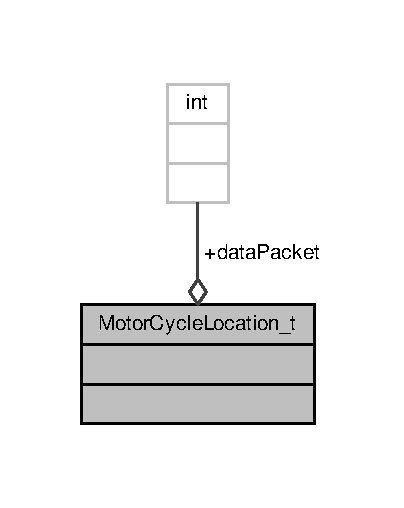
\includegraphics[width=194pt]{structMotorCycleLocation__t__coll__graph}
\end{center}
\end{figure}
\subsubsection*{Public Attributes}
\begin{DoxyCompactItemize}
\item 
\hyperlink{MotorcycleAwarenessSystemTypes_8hpp_ac0eb6e9beb8fa8db296c699fcc8494e6}{Data\-Packet\-\_\-t} \hyperlink{structMotorCycleLocation__t_a1f854587b19dbe91dffd637ce70be62e}{data\-Packet}
\begin{DoxyCompactList}\small\item\em V2\-V communication data packet. \end{DoxyCompactList}\end{DoxyCompactItemize}


\subsubsection{Detailed Description}
Struct for the V2\-V data. 

Definition at line \hyperlink{MotorcycleAwarenessSystemTypes_8hpp_source_l00049}{49} of file \hyperlink{MotorcycleAwarenessSystemTypes_8hpp_source}{Motorcycle\-Awareness\-System\-Types.\-hpp}.



\subsubsection{Member Data Documentation}
\hypertarget{structMotorCycleLocation__t_a1f854587b19dbe91dffd637ce70be62e}{\index{Motor\-Cycle\-Location\-\_\-t@{Motor\-Cycle\-Location\-\_\-t}!data\-Packet@{data\-Packet}}
\index{data\-Packet@{data\-Packet}!MotorCycleLocation_t@{Motor\-Cycle\-Location\-\_\-t}}
\paragraph[{data\-Packet}]{\setlength{\rightskip}{0pt plus 5cm}{\bf Data\-Packet\-\_\-t} Motor\-Cycle\-Location\-\_\-t\-::data\-Packet}}\label{structMotorCycleLocation__t_a1f854587b19dbe91dffd637ce70be62e}


V2\-V communication data packet. 



Definition at line \hyperlink{MotorcycleAwarenessSystemTypes_8hpp_source_l00051}{51} of file \hyperlink{MotorcycleAwarenessSystemTypes_8hpp_source}{Motorcycle\-Awareness\-System\-Types.\-hpp}.



The documentation for this struct was generated from the following file\-:\begin{DoxyCompactItemize}
\item 
\hyperlink{MotorcycleAwarenessSystemTypes_8hpp}{Motorcycle\-Awareness\-System\-Types.\-hpp}\end{DoxyCompactItemize}

\hypertarget{structRadarSignal__t}{\section{Radar\-Signal\-\_\-t Struct Reference}
\label{structRadarSignal__t}\index{Radar\-Signal\-\_\-t@{Radar\-Signal\-\_\-t}}
}


Structure that emulates a Radar signal.  




{\ttfamily \#include $<$Motorcycle\-Awareness\-System\-Types.\-hpp$>$}



Collaboration diagram for Radar\-Signal\-\_\-t\-:\nopagebreak
\begin{figure}[H]
\begin{center}
\leavevmode
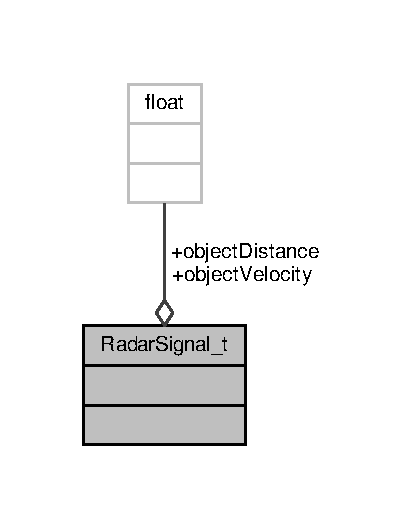
\includegraphics[width=158pt]{structRadarSignal__t__coll__graph}
\end{center}
\end{figure}
\subsection*{Public Attributes}
\begin{DoxyCompactItemize}
\item 
\hyperlink{MotorcycleAwarenessSystemTypes_8hpp_a6d34a01b51bff9b1cc17900d711a9b76}{Object\-Distance} \hyperlink{structRadarSignal__t_a79f6d1be92d835eba8fe0646c37d1053}{distance}
\begin{DoxyCompactList}\small\item\em Distance from sensed object to radar sensor. \end{DoxyCompactList}\item 
\hyperlink{MotorcycleAwarenessSystemTypes_8hpp_ae069b9d80ba548bc07502c05a1efaac0}{Object\-Velocity} \hyperlink{structRadarSignal__t_ac907ac4305b7d6c172661e95b030359d}{velocity}
\begin{DoxyCompactList}\small\item\em Velocity of sensed object. \end{DoxyCompactList}\end{DoxyCompactItemize}


\subsection{Detailed Description}
Structure that emulates a Radar signal. 

Definition at line 34 of file Motorcycle\-Awareness\-System\-Types.\-hpp.



\subsection{Member Data Documentation}
\hypertarget{structRadarSignal__t_a79f6d1be92d835eba8fe0646c37d1053}{\index{Radar\-Signal\-\_\-t@{Radar\-Signal\-\_\-t}!distance@{distance}}
\index{distance@{distance}!RadarSignal_t@{Radar\-Signal\-\_\-t}}
\subsubsection[{distance}]{\setlength{\rightskip}{0pt plus 5cm}{\bf Object\-Distance} Radar\-Signal\-\_\-t\-::distance}}\label{structRadarSignal__t_a79f6d1be92d835eba8fe0646c37d1053}


Distance from sensed object to radar sensor. 



Definition at line 36 of file Motorcycle\-Awareness\-System\-Types.\-hpp.

\hypertarget{structRadarSignal__t_ac907ac4305b7d6c172661e95b030359d}{\index{Radar\-Signal\-\_\-t@{Radar\-Signal\-\_\-t}!velocity@{velocity}}
\index{velocity@{velocity}!RadarSignal_t@{Radar\-Signal\-\_\-t}}
\subsubsection[{velocity}]{\setlength{\rightskip}{0pt plus 5cm}{\bf Object\-Velocity} Radar\-Signal\-\_\-t\-::velocity}}\label{structRadarSignal__t_ac907ac4305b7d6c172661e95b030359d}


Velocity of sensed object. 



Definition at line 37 of file Motorcycle\-Awareness\-System\-Types.\-hpp.



The documentation for this struct was generated from the following file\-:\begin{DoxyCompactItemize}
\item 
\hyperlink{MotorcycleAwarenessSystemTypes_8hpp}{Motorcycle\-Awareness\-System\-Types.\-hpp}\end{DoxyCompactItemize}

\hypertarget{structTurnSignal__t}{\subsection{Turn\-Signal\-\_\-t Struct Reference}
\label{structTurnSignal__t}\index{Turn\-Signal\-\_\-t@{Turn\-Signal\-\_\-t}}
}


{\ttfamily \#include $<$Motorcycle\-Awareness\-System\-Types.\-hpp$>$}



Collaboration diagram for Turn\-Signal\-\_\-t\-:\nopagebreak
\begin{figure}[H]
\begin{center}
\leavevmode
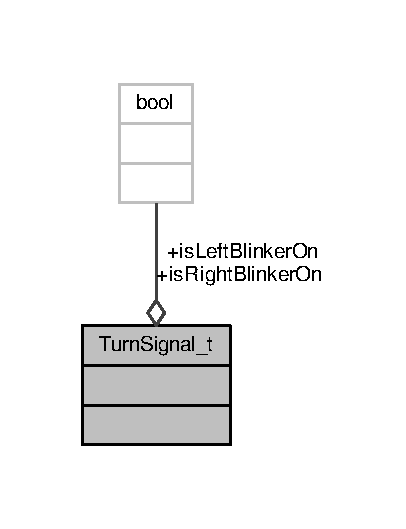
\includegraphics[width=195pt]{structTurnSignal__t__coll__graph}
\end{center}
\end{figure}
\subsubsection*{Public Attributes}
\begin{DoxyCompactItemize}
\item 
bool \hyperlink{structTurnSignal__t_a5b777c664220a398686d3a38661b4181}{is\-Right\-Blinker\-On}
\begin{DoxyCompactList}\small\item\em Right-\/hand-\/side blinker signal. \end{DoxyCompactList}\item 
bool \hyperlink{structTurnSignal__t_a7346ca64038ffb9b16cf2b22690dcae6}{is\-Left\-Blinker\-On}
\begin{DoxyCompactList}\small\item\em Left-\/hand-\/side blinker signal. \end{DoxyCompactList}\end{DoxyCompactItemize}


\subsubsection{Detailed Description}
Structure used to store the data coming from the turn-\/signal relay indicating the status of the blinker lights 

Definition at line \hyperlink{MotorcycleAwarenessSystemTypes_8hpp_source_l00016}{16} of file \hyperlink{MotorcycleAwarenessSystemTypes_8hpp_source}{Motorcycle\-Awareness\-System\-Types.\-hpp}.



\subsubsection{Member Data Documentation}
\hypertarget{structTurnSignal__t_a7346ca64038ffb9b16cf2b22690dcae6}{\index{Turn\-Signal\-\_\-t@{Turn\-Signal\-\_\-t}!is\-Left\-Blinker\-On@{is\-Left\-Blinker\-On}}
\index{is\-Left\-Blinker\-On@{is\-Left\-Blinker\-On}!TurnSignal_t@{Turn\-Signal\-\_\-t}}
\paragraph[{is\-Left\-Blinker\-On}]{\setlength{\rightskip}{0pt plus 5cm}bool Turn\-Signal\-\_\-t\-::is\-Left\-Blinker\-On}}\label{structTurnSignal__t_a7346ca64038ffb9b16cf2b22690dcae6}


Left-\/hand-\/side blinker signal. 



Definition at line \hyperlink{MotorcycleAwarenessSystemTypes_8hpp_source_l00019}{19} of file \hyperlink{MotorcycleAwarenessSystemTypes_8hpp_source}{Motorcycle\-Awareness\-System\-Types.\-hpp}.

\hypertarget{structTurnSignal__t_a5b777c664220a398686d3a38661b4181}{\index{Turn\-Signal\-\_\-t@{Turn\-Signal\-\_\-t}!is\-Right\-Blinker\-On@{is\-Right\-Blinker\-On}}
\index{is\-Right\-Blinker\-On@{is\-Right\-Blinker\-On}!TurnSignal_t@{Turn\-Signal\-\_\-t}}
\paragraph[{is\-Right\-Blinker\-On}]{\setlength{\rightskip}{0pt plus 5cm}bool Turn\-Signal\-\_\-t\-::is\-Right\-Blinker\-On}}\label{structTurnSignal__t_a5b777c664220a398686d3a38661b4181}


Right-\/hand-\/side blinker signal. 



Definition at line \hyperlink{MotorcycleAwarenessSystemTypes_8hpp_source_l00018}{18} of file \hyperlink{MotorcycleAwarenessSystemTypes_8hpp_source}{Motorcycle\-Awareness\-System\-Types.\-hpp}.



The documentation for this struct was generated from the following file\-:\begin{DoxyCompactItemize}
\item 
\hyperlink{MotorcycleAwarenessSystemTypes_8hpp}{Motorcycle\-Awareness\-System\-Types.\-hpp}\end{DoxyCompactItemize}

\section{File Documentation}
\hypertarget{main_8cpp}{\section{main.\-cpp File Reference}
\label{main_8cpp}\index{main.\-cpp@{main.\-cpp}}
}
{\ttfamily \#include \char`\"{}Motorcycle\-Awareness\-System.\-hpp\char`\"{}}\\*
{\ttfamily \#include \char`\"{}Motorcycle\-Awareness\-System\-Types.\-hpp\char`\"{}}\\*
{\ttfamily \#include $<$string$>$}\\*
{\ttfamily \#include $<$unistd.\-h$>$}\\*
Include dependency graph for main.\-cpp\-:\nopagebreak
\begin{figure}[H]
\begin{center}
\leavevmode
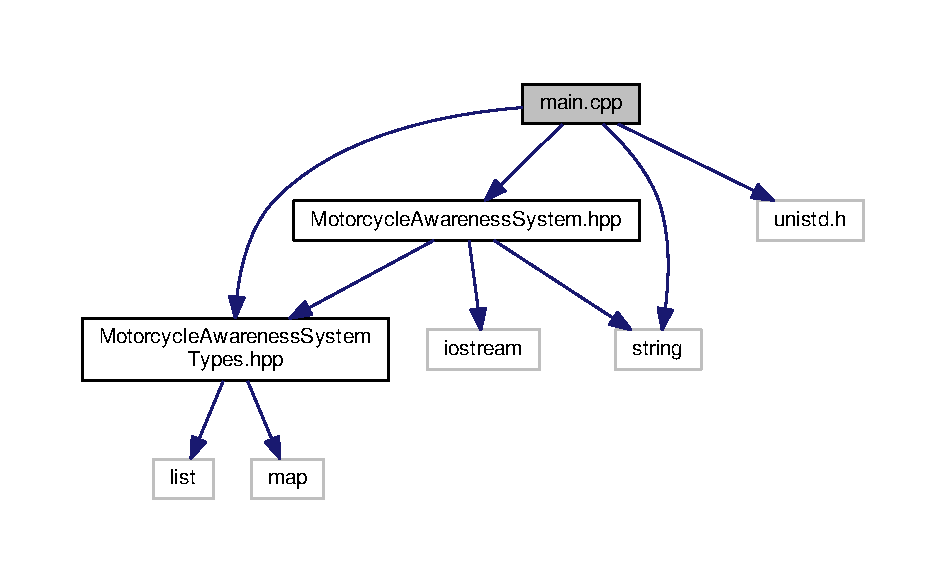
\includegraphics[width=350pt]{main_8cpp__incl}
\end{center}
\end{figure}
\subsection*{Functions}
\begin{DoxyCompactItemize}
\item 
int \hyperlink{main_8cpp_a840291bc02cba5474a4cb46a9b9566fe}{main} (void)
\end{DoxyCompactItemize}


\subsection{Function Documentation}
\hypertarget{main_8cpp_a840291bc02cba5474a4cb46a9b9566fe}{\index{main.\-cpp@{main.\-cpp}!main@{main}}
\index{main@{main}!main.cpp@{main.\-cpp}}
\subsubsection[{main}]{\setlength{\rightskip}{0pt plus 5cm}int main (
\begin{DoxyParamCaption}
\item[{void}]{}
\end{DoxyParamCaption}
)}}\label{main_8cpp_a840291bc02cba5474a4cb46a9b9566fe}


Definition at line 10 of file main.\-cpp.


\begin{DoxyCode}
11 \{
12     \textcolor{comment}{// Define mock signals}
13     \hyperlink{structCanSignal__t}{CanSignal\_t}* motorcycleCanSignal = \textcolor{keyword}{new} \hyperlink{structCanSignal__t}{CanSignal\_t};
14     \hyperlink{structCanSignal__t}{CanSignal\_t}* carCanSignal = \textcolor{keyword}{new} \hyperlink{structCanSignal__t}{CanSignal\_t};
15     \hyperlink{structRadarSignal__t}{RadarSignal\_t}* motorcycleRadarSignal = \textcolor{keyword}{new} \hyperlink{structRadarSignal__t}{RadarSignal\_t};
16     \hyperlink{structGpsSignal__t}{GpsSignal\_t}* motorcycleGpsSignal = \textcolor{keyword}{new} \hyperlink{structGpsSignal__t}{GpsSignal\_t};
17     \hyperlink{structGpsSignal__t}{GpsSignal\_t}* carGpsSignal = \textcolor{keyword}{new} \hyperlink{structGpsSignal__t}{GpsSignal\_t};;
18 
19     \textcolor{comment}{// Instantiate the Motorcycle Awareness System (MAS) for the motorcycle}
20     \hyperlink{classMotorcycleAwarenessSystem}{MotorcycleAwarenessSystem} MAS\_motorcycle( 
      \hyperlink{MotorcycleAwarenessSystemTypes_8hpp_a0c05c42b98a847f971385c81c2a81afaa39b983b1f7acfc4e7c900d77b0fded6a}{MOTORCYCLE} );
21     \textcolor{comment}{// Initialize the car MAS}
22     MAS\_motorcycle.Initialize( motorcycleCanSignal, carCanSignal, motorcycleRadarSignal,
23                                           motorcycleGpsSignal, carGpsSignal );
24 
25     \textcolor{comment}{// Instantiate the Motorcycle Awareness System (MAS) for the car}
26     \hyperlink{classMotorcycleAwarenessSystem}{MotorcycleAwarenessSystem} MAS\_car( \hyperlink{MotorcycleAwarenessSystemTypes_8hpp_a0c05c42b98a847f971385c81c2a81afaa5fc54ebcb1dd4bf1e1b93cbc77b57b40}{CAR} );
27     \textcolor{comment}{// Initialize the car MAS}
28     MAS\_car.Initialize( motorcycleCanSignal, carCanSignal, motorcycleRadarSignal,
29                                           motorcycleGpsSignal, carGpsSignal );
30 
31     \textcolor{comment}{// Run the MAS systems for the car & motorcycle}
32     \textcolor{keywordflow}{while} ( \textcolor{keyword}{true} )
33     \{
34         MAS\_motorcycle.MonitorConditions();
35         MAS\_car.MonitorConditions();
36         usleep(250);
37 
38 \textcolor{preprocessor}{#ifdef MAS\_DEBUG}
39 \textcolor{preprocessor}{}        std::cout << \textcolor{stringliteral}{"The MAS is running"} << std::endl;
40 \textcolor{preprocessor}{#endif}
41 \textcolor{preprocessor}{}    \}
42 
43     \textcolor{keywordflow}{return} 0;
44 \}
\end{DoxyCode}


Here is the call graph for this function\-:\nopagebreak
\begin{figure}[H]
\begin{center}
\leavevmode
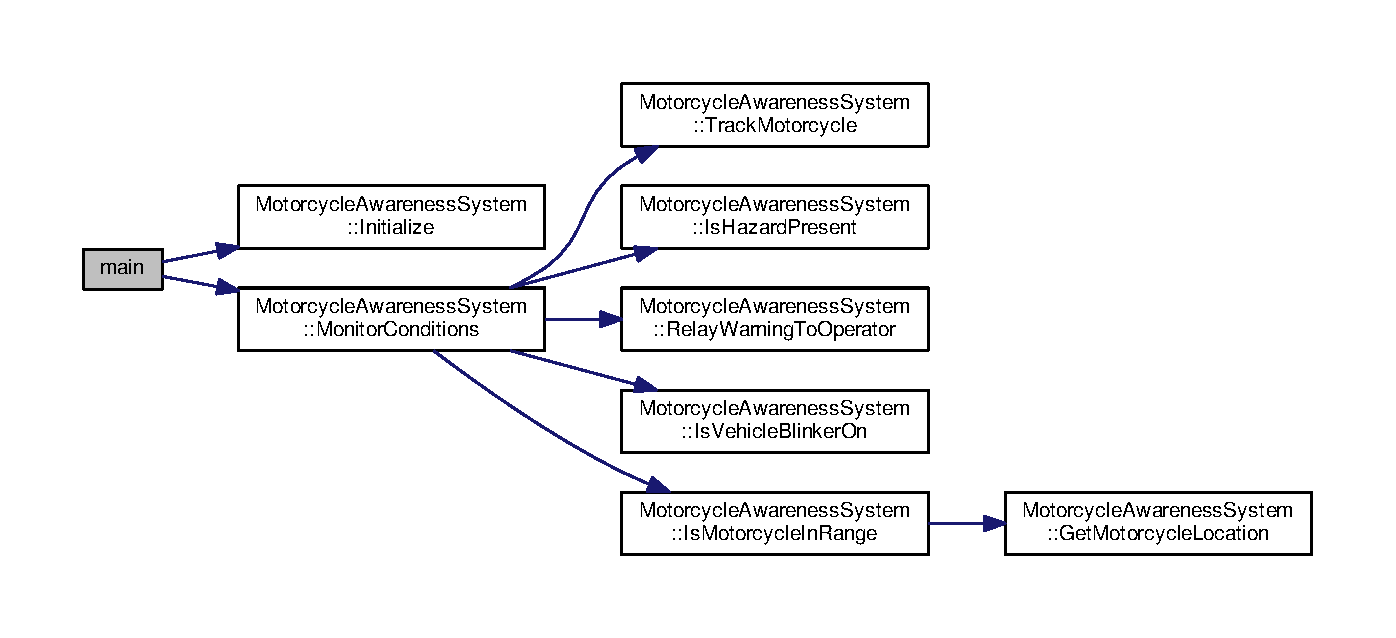
\includegraphics[width=350pt]{main_8cpp_a840291bc02cba5474a4cb46a9b9566fe_cgraph}
\end{center}
\end{figure}



\hypertarget{main_8cpp_source}{\subsection{main.\-cpp}
}

\begin{DoxyCode}
00001 \textcolor{preprocessor}{#include "\hyperlink{MotorcycleAwarenessSystem_8hpp}{MotorcycleAwarenessSystem.hpp}"}
00002 \textcolor{preprocessor}{#include "\hyperlink{MotorcycleAwarenessSystemTypes_8hpp}{MotorcycleAwarenessSystemTypes.hpp}"}
00003 
00004 \textcolor{preprocessor}{#ifdef MAS\_DEBUG}
00005 \textcolor{preprocessor}{}\textcolor{preprocessor}{#include <iostream>}
00006 \textcolor{preprocessor}{#endif}
00007 \textcolor{preprocessor}{}\textcolor{preprocessor}{#include <string>}
00008 \textcolor{preprocessor}{#include <unistd.h>}
00009 
\hypertarget{main_8cpp_source_l00010}{}\hyperlink{main_8cpp_a840291bc02cba5474a4cb46a9b9566fe}{00010} \textcolor{keywordtype}{int} \hyperlink{main_8cpp_a840291bc02cba5474a4cb46a9b9566fe}{main}( \textcolor{keywordtype}{void} )
00011 \{
00012     \textcolor{comment}{// Define mock signals}
00013     \hyperlink{structTurnSignal__t}{TurnSignal\_t}* motorcycleTurnSignal = \textcolor{keyword}{new} \hyperlink{structTurnSignal__t}{TurnSignal\_t};
00014     \hyperlink{structTurnSignal__t}{TurnSignal\_t}* carTurnSignal = \textcolor{keyword}{new} \hyperlink{structTurnSignal__t}{TurnSignal\_t};
00015     \hyperlink{structRadarSignal__t}{RadarSignal\_t}* motorcycleRadarSignal = \textcolor{keyword}{new} \hyperlink{structRadarSignal__t}{RadarSignal\_t};
00016     \hyperlink{structGpsSignal__t}{GpsSignal\_t}* motorcycleGpsSignal = \textcolor{keyword}{new} \hyperlink{structGpsSignal__t}{GpsSignal\_t};
00017     \hyperlink{structGpsSignal__t}{GpsSignal\_t}* carGpsSignal = \textcolor{keyword}{new} \hyperlink{structGpsSignal__t}{GpsSignal\_t};
00018 
00019     \textcolor{keywordtype}{bool} isSuccess = \textcolor{keyword}{false};
00020 
00021     \textcolor{comment}{// Instantiate the Motorcycle Awareness System (MAS) for the motorcycle}
00022     \hyperlink{classMotorcycleAwarenessSystem}{MotorcycleAwarenessSystem} MAS\_motorcycle( 
      \hyperlink{MotorcycleAwarenessSystemTypes_8hpp_a0c05c42b98a847f971385c81c2a81afaa39b983b1f7acfc4e7c900d77b0fded6a}{MOTORCYCLE} );
00023     \textcolor{comment}{// Initialize the car MAS}
00024     isSuccess = MAS\_motorcycle.\hyperlink{classMotorcycleAwarenessSystem_a341f27867c8d6aa0865040279ee246a9}{Initialize}( motorcycleTurnSignal, (
      \hyperlink{structTurnSignal__t}{TurnSignal\_t}*)NULL, motorcycleRadarSignal,
00025                                            motorcycleGpsSignal, carGpsSignal );
00026 \textcolor{preprocessor}{#ifdef MAS\_DEBUG}
00027 \textcolor{preprocessor}{}    \textcolor{keywordflow}{if} ( !isSuccess )
00028     \{
00029         std::cout << \textcolor{stringliteral}{"MAS initialization for the motorcycle failed"} << std::endl;
00030     \}
00031 \textcolor{preprocessor}{#endif}
00032 \textcolor{preprocessor}{}
00033     \textcolor{comment}{// Instantiate the Motorcycle Awareness System (MAS) for the car}
00034     \hyperlink{classMotorcycleAwarenessSystem}{MotorcycleAwarenessSystem} MAS\_car( \hyperlink{MotorcycleAwarenessSystemTypes_8hpp_a0c05c42b98a847f971385c81c2a81afaa5fc54ebcb1dd4bf1e1b93cbc77b57b40}{CAR} );
00035     \textcolor{comment}{// Initialize the car MAS}
00036     isSuccess =  MAS\_car.\hyperlink{classMotorcycleAwarenessSystem_a341f27867c8d6aa0865040279ee246a9}{Initialize}( (\hyperlink{structTurnSignal__t}{TurnSignal\_t}*)NULL, carTurnSignal, 
      motorcycleRadarSignal,
00037                                      motorcycleGpsSignal, carGpsSignal );
00038 \textcolor{preprocessor}{#ifdef MAS\_DEBUG}
00039 \textcolor{preprocessor}{}    \textcolor{keywordflow}{if} ( !isSuccess )
00040     \{
00041         std::cout << \textcolor{stringliteral}{"MAS initialization for the car failed"} << std::endl;
00042     \}
00043 \textcolor{preprocessor}{#endif}
00044 \textcolor{preprocessor}{}
00045     \textcolor{comment}{// Run the MAS systems for the car & motorcycle only if the systems were}
00046     \textcolor{comment}{// initialized successfully}
00047     \textcolor{keywordflow}{if} ( isSuccess )
00048     \{
00049         \textcolor{keywordflow}{while} ( \textcolor{keyword}{true} )
00050         \{
00051             MAS\_motorcycle.\hyperlink{classMotorcycleAwarenessSystem_afb19e832c17d43941d9ed6c4f4435a2e}{MonitorConditions}();
00052             MAS\_car.\hyperlink{classMotorcycleAwarenessSystem_afb19e832c17d43941d9ed6c4f4435a2e}{MonitorConditions}();
00053             usleep(250);
00054 
00055 \textcolor{preprocessor}{#ifdef MAS\_DEBUG}
00056 \textcolor{preprocessor}{}            std::cout << \textcolor{stringliteral}{"The MAS is running"} << std::endl;
00057 \textcolor{preprocessor}{#endif}
00058 \textcolor{preprocessor}{}        \}
00059     \}
00060 
00061     \textcolor{keywordflow}{return} 0;
00062 \}
\end{DoxyCode}

\hypertarget{mainpage_8dox}{\subsection{mainpage.\-dox File Reference}
\label{mainpage_8dox}\index{mainpage.\-dox@{mainpage.\-dox}}
}

\hypertarget{MotorcycleAwarenessSystem_8cpp}{\section{Motorcycle\-Awareness\-System.\-cpp File Reference}
\label{MotorcycleAwarenessSystem_8cpp}\index{Motorcycle\-Awareness\-System.\-cpp@{Motorcycle\-Awareness\-System.\-cpp}}
}
{\ttfamily \#include \char`\"{}Motorcycle\-Awareness\-System.\-hpp\char`\"{}}\\*
{\ttfamily \#include \char`\"{}Motorcycle\-Awareness\-System\-Types.\-hpp\char`\"{}}\\*
{\ttfamily \#include $<$list$>$}\\*
{\ttfamily \#include $<$map$>$}\\*
Include dependency graph for Motorcycle\-Awareness\-System.\-cpp\-:\nopagebreak
\begin{figure}[H]
\begin{center}
\leavevmode
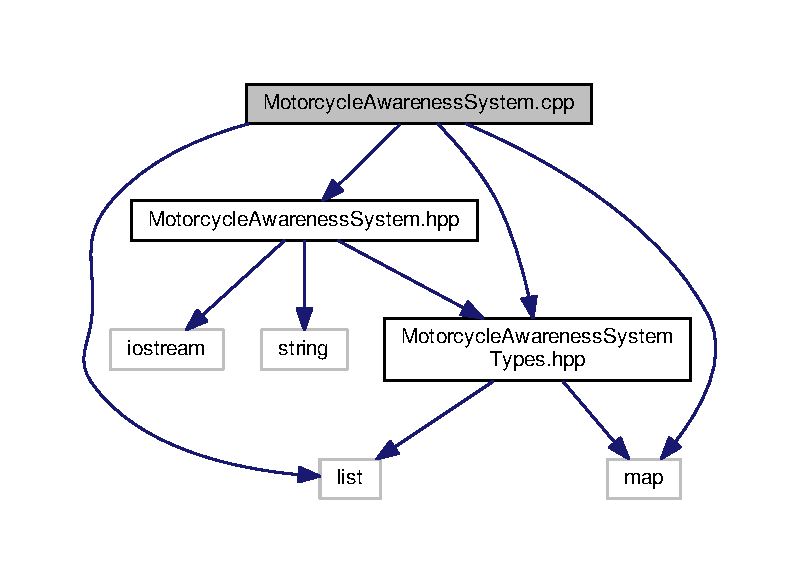
\includegraphics[width=350pt]{MotorcycleAwarenessSystem_8cpp__incl}
\end{center}
\end{figure}

\hypertarget{MotorcycleAwarenessSystem_8cpp_source}{\subsection{Motorcycle\-Awareness\-System.\-cpp}
}

\begin{DoxyCode}
00001 \textcolor{preprocessor}{#include "\hyperlink{MotorcycleAwarenessSystem_8hpp}{MotorcycleAwarenessSystem.hpp}"}
00007 \textcolor{preprocessor}{#include "\hyperlink{MotorcycleAwarenessSystemTypes_8hpp}{MotorcycleAwarenessSystemTypes.hpp}"}
00008 
00009 \textcolor{preprocessor}{#include <list>}
00010 \textcolor{preprocessor}{#include <map>}
00011 
\hypertarget{MotorcycleAwarenessSystem_8cpp_source_l00013}{}\hyperlink{classMotorcycleAwarenessSystem_ab0fb3823809dc056fecc82cc72a80a55}{00013} \hyperlink{classMotorcycleAwarenessSystem_ab0fb3823809dc056fecc82cc72a80a55}{MotorcycleAwarenessSystem::MotorcycleAwarenessSystem}( 
      \hyperlink{MotorcycleAwarenessSystemTypes_8hpp_a0c05c42b98a847f971385c81c2a81afa}{VehicleType} vehicleType )
00014     :vehicleType( vehicleType )
00015 \{
00016     \textcolor{comment}{// Do nothing}
00017 \}
00018 
\hypertarget{MotorcycleAwarenessSystem_8cpp_source_l00020}{}\hyperlink{classMotorcycleAwarenessSystem_a89ce16a722b3575e1415cbe9c7eedbd3}{00020} \hyperlink{classMotorcycleAwarenessSystem_a89ce16a722b3575e1415cbe9c7eedbd3}{MotorcycleAwarenessSystem::~MotorcycleAwarenessSystem}(
       \textcolor{keywordtype}{void} )
00021 \{
00022     \textcolor{comment}{// Do nothing}
00023 \}
00024 
\hypertarget{MotorcycleAwarenessSystem_8cpp_source_l00026}{}\hyperlink{classMotorcycleAwarenessSystem_a826b6c2286c494c8aca3a47e6430b3ff}{00026} \textcolor{keywordtype}{void} \hyperlink{classMotorcycleAwarenessSystem_a826b6c2286c494c8aca3a47e6430b3ff}{MotorcycleAwarenessSystem::Initialize}( 
      \hyperlink{structTurnSignal__t}{TurnSignal\_t}* motorcycleTurnSignal, \hyperlink{structTurnSignal__t}{TurnSignal\_t}* carTurnSignal,
00027                                             \hyperlink{structRadarSignal__t}{RadarSignal\_t}* motorcycleRadarSignal, 
      \hyperlink{structGpsSignal__t}{GpsSignal\_t}* motorcycleGpsSignal,
00028                                             \hyperlink{structGpsSignal__t}{GpsSignal\_t}* carGpsSignal  )
00029 \{
00030     \textcolor{comment}{// Initialize the motorcycle radar signal}
00031     this->motorcycleRadarSignal = \hyperlink{classMotorcycleAwarenessSystem_a0744e71b9f440a86f5078c876ba7629b}{motorcycleRadarSignal};
00032 
00033     \textcolor{comment}{// Initialize the turn signal map}
00034     \hyperlink{classMotorcycleAwarenessSystem_a43fde090639a3a58fc5bbf8bafc966f7}{turnSignal}[\hyperlink{MotorcycleAwarenessSystemTypes_8hpp_a0c05c42b98a847f971385c81c2a81afaa39b983b1f7acfc4e7c900d77b0fded6a}{MOTORCYCLE}] = motorcycleTurnSignal;
00035     \hyperlink{classMotorcycleAwarenessSystem_a43fde090639a3a58fc5bbf8bafc966f7}{turnSignal}[\hyperlink{MotorcycleAwarenessSystemTypes_8hpp_a0c05c42b98a847f971385c81c2a81afaa5fc54ebcb1dd4bf1e1b93cbc77b57b40}{CAR}] = carTurnSignal;
00036 
00037     \textcolor{comment}{// Initialize the GPS signals}
00038     this->motorcycleGpsSignal = \hyperlink{classMotorcycleAwarenessSystem_ab281a3993b574923b2f379ed0477b2d4}{motorcycleGpsSignal};
00039     this->motorcycleGpsSignal = \hyperlink{classMotorcycleAwarenessSystem_ab281a3993b574923b2f379ed0477b2d4}{motorcycleGpsSignal};
00040 \}
00041 
\hypertarget{MotorcycleAwarenessSystem_8cpp_source_l00043}{}\hyperlink{classMotorcycleAwarenessSystem_afb19e832c17d43941d9ed6c4f4435a2e}{00043} \textcolor{keywordtype}{void} \hyperlink{classMotorcycleAwarenessSystem_afb19e832c17d43941d9ed6c4f4435a2e}{MotorcycleAwarenessSystem::MonitorConditions}( \textcolor{keywordtype}{void} )
00044 \{
00045     \textcolor{keywordflow}{if} ( \hyperlink{MotorcycleAwarenessSystemTypes_8hpp_a0c05c42b98a847f971385c81c2a81afaa39b983b1f7acfc4e7c900d77b0fded6a}{MOTORCYCLE} == \hyperlink{classMotorcycleAwarenessSystem_a977b2085bfbf6a62902bf2d80160e6d2}{vehicleType} )
00046     \{
00047         \textcolor{comment}{// Track the motorcycle}
00048         \hyperlink{classMotorcycleAwarenessSystem_a4e6eec23ec46e24ee377a3c94e15eba4}{TrackMotorcycle}();
00049         \textcolor{comment}{// Check for hazards}
00050         \textcolor{keywordflow}{if} ( \hyperlink{classMotorcycleAwarenessSystem_a35d59c8299b0d5ef43c10306cc7f2ee1}{IsHazardPresent}() == \textcolor{keyword}{true} )
00051         \{
00052             \textcolor{comment}{// Warn the motorcycle operator}
00053             \hyperlink{classMotorcycleAwarenessSystem_aec5e4731c6bf0789821ba2793918e3ee}{RelayWarningToOperator}();
00054         \}
00055     \}
00056     \textcolor{comment}{// vehicleType == CAR}
00057     \textcolor{keywordflow}{else}
00058     \{
00059         \textcolor{comment}{// Check for hazards}
00060         \textcolor{keywordflow}{if} ( (\hyperlink{classMotorcycleAwarenessSystem_a9c3f98a014b0af39fa120f478eb5f348}{IsVehicleBlinkerOn}() == \textcolor{keyword}{true}) && (
      \hyperlink{classMotorcycleAwarenessSystem_a239655aca9c875b1dbbad3ce155c7892}{IsMotorcycleInRange}() == \textcolor{keyword}{true}) )
00061         \{
00062             \textcolor{comment}{// Relay message to the car driver}
00063             \hyperlink{classMotorcycleAwarenessSystem_aec5e4731c6bf0789821ba2793918e3ee}{RelayWarningToOperator}();
00064         \}
00065     \}
00066 \}
00067 
\hypertarget{MotorcycleAwarenessSystem_8cpp_source_l00069}{}\hyperlink{classMotorcycleAwarenessSystem_a9c3f98a014b0af39fa120f478eb5f348}{00069} \textcolor{keywordtype}{bool} \hyperlink{classMotorcycleAwarenessSystem_a9c3f98a014b0af39fa120f478eb5f348}{MotorcycleAwarenessSystem::IsVehicleBlinkerOn}( \textcolor{keywordtype}{void} )
00070 \{
00071     \textcolor{keywordtype}{bool} isBlinkerOn = \textcolor{keyword}{false};
00072 
00073     \textcolor{keywordflow}{if} ( this->\hyperlink{classMotorcycleAwarenessSystem_a43fde090639a3a58fc5bbf8bafc966f7}{turnSignal}[\hyperlink{classMotorcycleAwarenessSystem_a977b2085bfbf6a62902bf2d80160e6d2}{vehicleType}]->isRightBlinkerOn ||
00074          this->\hyperlink{classMotorcycleAwarenessSystem_a43fde090639a3a58fc5bbf8bafc966f7}{turnSignal}[\hyperlink{classMotorcycleAwarenessSystem_a977b2085bfbf6a62902bf2d80160e6d2}{vehicleType}]->isLeftBlinkerOn )
00075     \{
00076         isBlinkerOn = \textcolor{keyword}{true};
00077     \}
00078 
00079     \textcolor{keywordflow}{return} isBlinkerOn;
00080 \}
00081 
\hypertarget{MotorcycleAwarenessSystem_8cpp_source_l00083}{}\hyperlink{classMotorcycleAwarenessSystem_a239655aca9c875b1dbbad3ce155c7892}{00083} \textcolor{keywordtype}{bool} \hyperlink{classMotorcycleAwarenessSystem_a239655aca9c875b1dbbad3ce155c7892}{MotorcycleAwarenessSystem::IsMotorcycleInRange}( \textcolor{keywordtype}{void} )
00084 \{
00085     \textcolor{keywordtype}{bool} isInRange = \textcolor{keyword}{false};
00086 
00087     \textcolor{comment}{// Determine where the motorcycle is relative to the car using the GPS signals}
00088     \textcolor{keywordflow}{if} ( abs( (this->\hyperlink{classMotorcycleAwarenessSystem_a9a8185e00b60d0be58bfa76166063128}{carGpsSignal}->\hyperlink{structGpsSignal__t_a6f7bd3c500b55923ab335ada4b6b26eb}{x}) - (this->motorcycleGpsSignal->x) ) <= 
      \hyperlink{classMotorcycleAwarenessSystem_a131c99d85b78020f94fe14bd397f3a6e}{SAFETY\_ZONE} &&
00089          abs( (this->\hyperlink{classMotorcycleAwarenessSystem_a9a8185e00b60d0be58bfa76166063128}{carGpsSignal}->\hyperlink{structGpsSignal__t_ab9e083be189fc842ed7aa4fdc978e94e}{y}) - (this->motorcycleGpsSignal->y) ) <= 
      \hyperlink{classMotorcycleAwarenessSystem_a131c99d85b78020f94fe14bd397f3a6e}{SAFETY\_ZONE} )
00090     \{
00091         isInRange = \textcolor{keyword}{true};
00092     \}
00093     \textcolor{keywordflow}{else}
00094     \{
00095         \textcolor{comment}{// Analyze the V2V data for a threat}
00096         \hyperlink{structMotorCycleLocation__t}{MotorCycleLocation\_t} motorCycleLocation = 
      \hyperlink{classMotorcycleAwarenessSystem_a840a5bc17d75276ecdb3a39d7aaf4109}{GetMotorcycleLocation}();
00098     \}
00099 
00100     \textcolor{keywordflow}{return} isInRange;
00101 \}
00102 
\hypertarget{MotorcycleAwarenessSystem_8cpp_source_l00105}{}\hyperlink{classMotorcycleAwarenessSystem_a35d59c8299b0d5ef43c10306cc7f2ee1}{00105} \textcolor{keywordtype}{bool} \hyperlink{classMotorcycleAwarenessSystem_a35d59c8299b0d5ef43c10306cc7f2ee1}{MotorcycleAwarenessSystem::IsHazardPresent}( \textcolor{keywordtype}{void} )
00106 \{
00107     \textcolor{keywordtype}{bool} isHazardPresent = \textcolor{keyword}{false};
00108 
00109     \textcolor{keywordflow}{if} ( abs( this->\hyperlink{classMotorcycleAwarenessSystem_a0744e71b9f440a86f5078c876ba7629b}{motorcycleRadarSignal}->\hyperlink{structRadarSignal__t_a96938fbfb77f208743a36d3f8b37cccb}{objectDistance} ) <= 
      \hyperlink{classMotorcycleAwarenessSystem_a131c99d85b78020f94fe14bd397f3a6e}{SAFETY\_ZONE} )
00110     \{
00111         isHazardPresent = \textcolor{keyword}{true};
00112     \}
00113 
00114     \textcolor{keywordflow}{return} isHazardPresent;
00115 \}
00116 
\hypertarget{MotorcycleAwarenessSystem_8cpp_source_l00118}{}\hyperlink{classMotorcycleAwarenessSystem_a4e6eec23ec46e24ee377a3c94e15eba4}{00118} \textcolor{keywordtype}{void} \hyperlink{classMotorcycleAwarenessSystem_a4e6eec23ec46e24ee377a3c94e15eba4}{MotorcycleAwarenessSystem::TrackMotorcycle}( \textcolor{keywordtype}{void} )
00119 \{
00120     \textcolor{comment}{// Push the motorcycle's GPS location onto the list}
00121     \hyperlink{classMotorcycleAwarenessSystem_af6becfeb1d11b467cb80a94a8e6940ac}{motorcycleLocation}.push\_front( *\hyperlink{classMotorcycleAwarenessSystem_ab281a3993b574923b2f379ed0477b2d4}{motorcycleGpsSignal} );
00122 \}
00123 
\hypertarget{MotorcycleAwarenessSystem_8cpp_source_l00125}{}\hyperlink{classMotorcycleAwarenessSystem_aec5e4731c6bf0789821ba2793918e3ee}{00125} \textcolor{keywordtype}{void} \hyperlink{classMotorcycleAwarenessSystem_aec5e4731c6bf0789821ba2793918e3ee}{MotorcycleAwarenessSystem::RelayWarningToOperator}( \textcolor{keywordtype}{
      void} )
00126 \{
00127     \textcolor{comment}{// Assemble the message to be sent}
00128     \hyperlink{structBlueToothMessage__t}{BlueToothMessage\_t} blueToothMessage;
00129     blueToothMessage.\hyperlink{structBlueToothMessage__t_a2dd315aa1cba1d2d3045e26b9f171e61}{isHazardPresent} = \textcolor{keyword}{true};
00130     \textcolor{comment}{// Dummy message}
00131     blueToothMessage.\hyperlink{structBlueToothMessage__t_ab872789a32f068dae8bcf77122256b78}{dataBuffer}[0] = 0x2015;
00132 
00134 \}
00135 
00136 \textcolor{comment}{// Method to Get motorcycle's location via V2V communication}
\hypertarget{MotorcycleAwarenessSystem_8cpp_source_l00137}{}\hyperlink{classMotorcycleAwarenessSystem_a840a5bc17d75276ecdb3a39d7aaf4109}{00137} \hyperlink{structMotorCycleLocation__t}{MotorCycleLocation\_t} 
      \hyperlink{classMotorcycleAwarenessSystem_a840a5bc17d75276ecdb3a39d7aaf4109}{MotorcycleAwarenessSystem::GetMotorcycleLocation}( \textcolor{keywordtype}{void} )
00138 \{
00139     \textcolor{comment}{// Dummy motorcycle location from V2V communication}
00140     \hyperlink{structMotorCycleLocation__t}{MotorCycleLocation\_t} motorCycleLocation;
00142 
00143     \textcolor{keywordflow}{return} motorCycleLocation;
00144 \}
\end{DoxyCode}

\hypertarget{MotorcycleAwarenessSystem_8hpp}{\section{Motorcycle\-Awareness\-System.\-hpp File Reference}
\label{MotorcycleAwarenessSystem_8hpp}\index{Motorcycle\-Awareness\-System.\-hpp@{Motorcycle\-Awareness\-System.\-hpp}}
}
{\ttfamily \#include \char`\"{}Motorcycle\-Awareness\-System\-Types.\-hpp\char`\"{}}\\*
{\ttfamily \#include $<$string$>$}\\*
{\ttfamily \#include $<$iostream$>$}\\*
Include dependency graph for Motorcycle\-Awareness\-System.\-hpp\-:\nopagebreak
\begin{figure}[H]
\begin{center}
\leavevmode
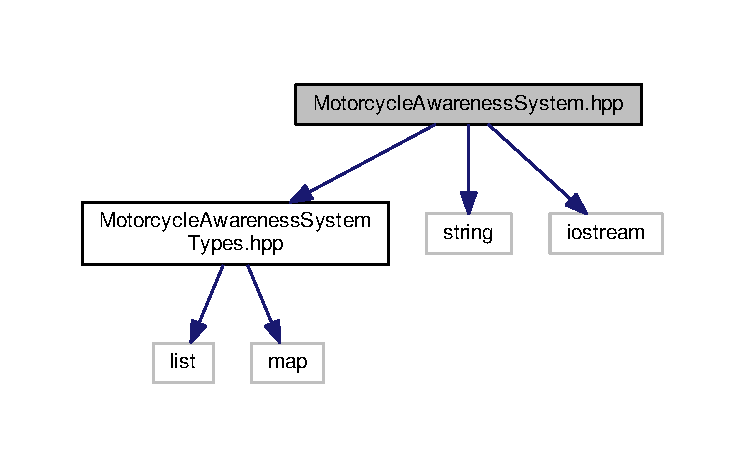
\includegraphics[width=350pt]{MotorcycleAwarenessSystem_8hpp__incl}
\end{center}
\end{figure}
This graph shows which files directly or indirectly include this file\-:\nopagebreak
\begin{figure}[H]
\begin{center}
\leavevmode
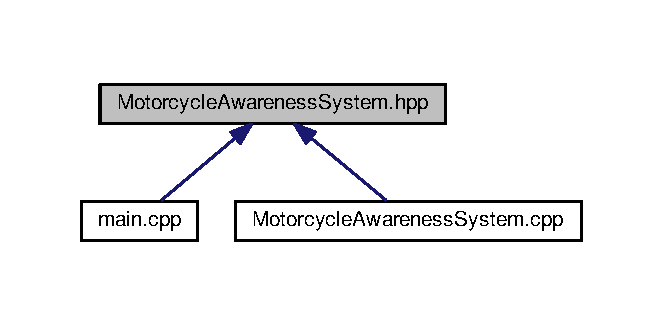
\includegraphics[width=319pt]{MotorcycleAwarenessSystem_8hpp__dep__incl}
\end{center}
\end{figure}
\subsection*{Classes}
\begin{DoxyCompactItemize}
\item 
class \hyperlink{classMotorcycleAwarenessSystem}{Motorcycle\-Awareness\-System}
\begin{DoxyCompactList}\small\item\em Class declaration for the Motorcycle Awareness System (M\-A\-S) \end{DoxyCompactList}\end{DoxyCompactItemize}

\hypertarget{MotorcycleAwarenessSystem_8hpp_source}{\section{Motorcycle\-Awareness\-System.\-hpp}
}

\begin{DoxyCode}
00001 \textcolor{preprocessor}{#ifndef MOTORCYCLEAWARENESSSYSTEM\_HPP}
00005 \textcolor{preprocessor}{}\textcolor{preprocessor}{#define MOTORCYCLEAWARENESSSYSTEM\_HPP}
00006 \textcolor{preprocessor}{}
00007 \textcolor{preprocessor}{#include "\hyperlink{MotorcycleAwarenessSystemTypes_8hpp}{MotorcycleAwarenessSystemTypes.hpp}"}
00008 
00009 \textcolor{preprocessor}{#include <string>}
00010 \textcolor{preprocessor}{#include <iostream>}
00011 
\hypertarget{MotorcycleAwarenessSystem_8hpp_source_l00012}{}\hyperlink{classMotorcycleAwarenessSystem}{00012} \textcolor{keyword}{class }\hyperlink{classMotorcycleAwarenessSystem}{MotorcycleAwarenessSystem}
00013 \{
00014     \textcolor{keyword}{public}:
00015         \hyperlink{classMotorcycleAwarenessSystem_ab0fb3823809dc056fecc82cc72a80a55}{MotorcycleAwarenessSystem}( \hyperlink{MotorcycleAwarenessSystemTypes_8hpp_a0c05c42b98a847f971385c81c2a81afa}{VehicleType} 
      \hyperlink{classMotorcycleAwarenessSystem_a977b2085bfbf6a62902bf2d80160e6d2}{vehicleType} );
00016         \hyperlink{classMotorcycleAwarenessSystem_a89ce16a722b3575e1415cbe9c7eedbd3}{~MotorcycleAwarenessSystem}( \textcolor{keywordtype}{void} );
00017         \textcolor{keywordtype}{void} \hyperlink{classMotorcycleAwarenessSystem_a55f1ea16b6311120ea42b460fb8b3a71}{Initialize}( \hyperlink{structCanSignal__t}{CanSignal\_t}* motorcycleCanSignal, 
      \hyperlink{structCanSignal__t}{CanSignal\_t}* carCanSignal,
00018                          \hyperlink{structRadarSignal__t}{RadarSignal\_t}* \hyperlink{classMotorcycleAwarenessSystem_a0744e71b9f440a86f5078c876ba7629b}{motorcycleRadarSignal}, 
      \hyperlink{structGpsSignal__t}{GpsSignal\_t}* \hyperlink{classMotorcycleAwarenessSystem_ab281a3993b574923b2f379ed0477b2d4}{motorcycleGpsSignal},
00019                          \hyperlink{structGpsSignal__t}{GpsSignal\_t}* \hyperlink{classMotorcycleAwarenessSystem_a9a8185e00b60d0be58bfa76166063128}{carGpsSignal} );
00020         \textcolor{keywordtype}{void} \hyperlink{classMotorcycleAwarenessSystem_afb19e832c17d43941d9ed6c4f4435a2e}{MonitorConditions}( \textcolor{keywordtype}{void} );
00021 
00022     \textcolor{keyword}{private}:
\hypertarget{MotorcycleAwarenessSystem_8hpp_source_l00023}{}\hyperlink{classMotorcycleAwarenessSystem_af6becfeb1d11b467cb80a94a8e6940ac}{00023}         std::list<GpsSignal\_t> \hyperlink{classMotorcycleAwarenessSystem_af6becfeb1d11b467cb80a94a8e6940ac}{motorcycleLocation}; 
\hypertarget{MotorcycleAwarenessSystem_8hpp_source_l00024}{}\hyperlink{classMotorcycleAwarenessSystem_abe0296f34c0ca2857a94659dfdc5801c}{00024}         \textcolor{keyword}{static} \textcolor{keyword}{const} \textcolor{keywordtype}{unsigned} \textcolor{keywordtype}{int} \hyperlink{classMotorcycleAwarenessSystem_abe0296f34c0ca2857a94659dfdc5801c}{DANGER\_ZONE} = 15U; 
\hypertarget{MotorcycleAwarenessSystem_8hpp_source_l00025}{}\hyperlink{classMotorcycleAwarenessSystem_a977b2085bfbf6a62902bf2d80160e6d2}{00025}         \hyperlink{MotorcycleAwarenessSystemTypes_8hpp_a0c05c42b98a847f971385c81c2a81afa}{VehicleType} \hyperlink{classMotorcycleAwarenessSystem_a977b2085bfbf6a62902bf2d80160e6d2}{vehicleType}; 
\hypertarget{MotorcycleAwarenessSystem_8hpp_source_l00026}{}\hyperlink{classMotorcycleAwarenessSystem_a2d8ac602ae24dcf38aaa95a42ffb4e1f}{00026}         std::map<VehicleType, CanSignal\_t*> \hyperlink{classMotorcycleAwarenessSystem_a2d8ac602ae24dcf38aaa95a42ffb4e1f}{canSignal}; 
\hypertarget{MotorcycleAwarenessSystem_8hpp_source_l00027}{}\hyperlink{classMotorcycleAwarenessSystem_a0744e71b9f440a86f5078c876ba7629b}{00027}         \hyperlink{structRadarSignal__t}{RadarSignal\_t}* \hyperlink{classMotorcycleAwarenessSystem_a0744e71b9f440a86f5078c876ba7629b}{motorcycleRadarSignal}; 
\hypertarget{MotorcycleAwarenessSystem_8hpp_source_l00028}{}\hyperlink{classMotorcycleAwarenessSystem_ab281a3993b574923b2f379ed0477b2d4}{00028}         \hyperlink{structGpsSignal__t}{GpsSignal\_t}* \hyperlink{classMotorcycleAwarenessSystem_ab281a3993b574923b2f379ed0477b2d4}{motorcycleGpsSignal}; 
\hypertarget{MotorcycleAwarenessSystem_8hpp_source_l00029}{}\hyperlink{classMotorcycleAwarenessSystem_a9a8185e00b60d0be58bfa76166063128}{00029}         \hyperlink{structGpsSignal__t}{GpsSignal\_t}* \hyperlink{classMotorcycleAwarenessSystem_a9a8185e00b60d0be58bfa76166063128}{carGpsSignal}; 
00030 
00031         \textcolor{keywordtype}{bool} \hyperlink{classMotorcycleAwarenessSystem_a9c3f98a014b0af39fa120f478eb5f348}{IsVehicleBlinkerOn}( \textcolor{keywordtype}{void} );
00032         \textcolor{keywordtype}{bool} \hyperlink{classMotorcycleAwarenessSystem_a239655aca9c875b1dbbad3ce155c7892}{IsMotorcycleInRange}( \textcolor{keywordtype}{void} );
00033         \textcolor{keywordtype}{bool} \hyperlink{classMotorcycleAwarenessSystem_a35d59c8299b0d5ef43c10306cc7f2ee1}{IsHazardPresent}( \textcolor{keywordtype}{void} );
00034         \textcolor{keywordtype}{void} \hyperlink{classMotorcycleAwarenessSystem_a4e6eec23ec46e24ee377a3c94e15eba4}{TrackMotorcycle}( \textcolor{keywordtype}{void} );
00035         \textcolor{keywordtype}{void} \hyperlink{classMotorcycleAwarenessSystem_aec5e4731c6bf0789821ba2793918e3ee}{RelayWarningToOperator}( \textcolor{keywordtype}{void} );
00036         \hyperlink{structMotorCycleLocation__t}{MotorCycleLocation\_t} \hyperlink{classMotorcycleAwarenessSystem_a840a5bc17d75276ecdb3a39d7aaf4109}{GetMotorcycleLocation}( \textcolor{keywordtype}{void} );
00037 \};
00038 \textcolor{preprocessor}{#endif}
\end{DoxyCode}

\hypertarget{MotorcycleAwarenessSystemTypes_8hpp}{\section{Motorcycle\-Awareness\-System\-Types.\-hpp File Reference}
\label{MotorcycleAwarenessSystemTypes_8hpp}\index{Motorcycle\-Awareness\-System\-Types.\-hpp@{Motorcycle\-Awareness\-System\-Types.\-hpp}}
}
{\ttfamily \#include $<$list$>$}\\*
{\ttfamily \#include $<$map$>$}\\*
Include dependency graph for Motorcycle\-Awareness\-System\-Types.\-hpp\-:\nopagebreak
\begin{figure}[H]
\begin{center}
\leavevmode
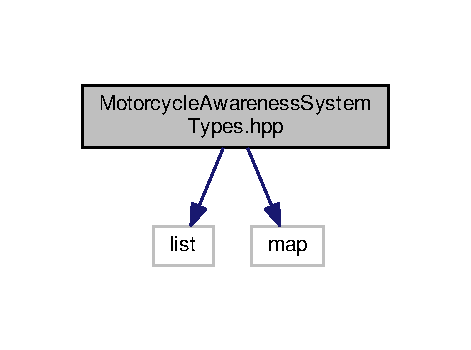
\includegraphics[width=226pt]{MotorcycleAwarenessSystemTypes_8hpp__incl}
\end{center}
\end{figure}
This graph shows which files directly or indirectly include this file\-:\nopagebreak
\begin{figure}[H]
\begin{center}
\leavevmode
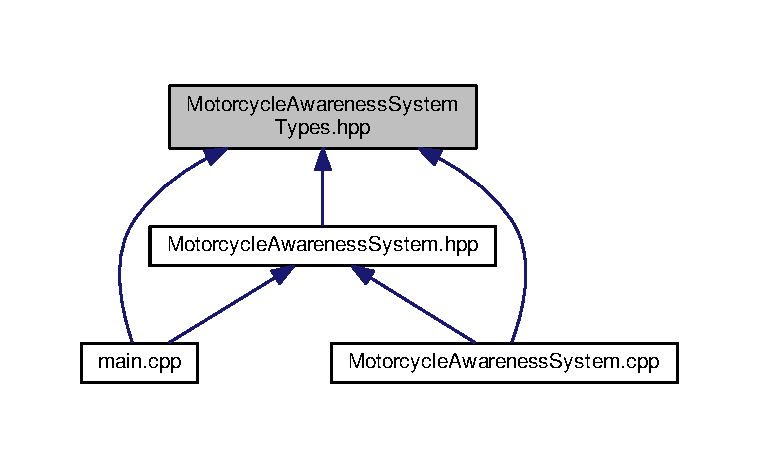
\includegraphics[width=350pt]{MotorcycleAwarenessSystemTypes_8hpp__dep__incl}
\end{center}
\end{figure}
\subsection*{Classes}
\begin{DoxyCompactItemize}
\item 
struct \hyperlink{structCanSignal__t}{Can\-Signal\-\_\-t}
\begin{DoxyCompactList}\small\item\em Structure that emulates a C\-A\-N bus signal. \end{DoxyCompactList}\item 
struct \hyperlink{structGpsSignal__t}{Gps\-Signal\-\_\-t}
\begin{DoxyCompactList}\small\item\em Structure that emulates a G\-P\-S signal. \end{DoxyCompactList}\item 
struct \hyperlink{structRadarSignal__t}{Radar\-Signal\-\_\-t}
\begin{DoxyCompactList}\small\item\em Structure that emulates a Radar signal. \end{DoxyCompactList}\item 
struct \hyperlink{structBlueToothMessage__t}{Blue\-Tooth\-Message\-\_\-t}
\begin{DoxyCompactList}\small\item\em Struct for bluetooth message. \end{DoxyCompactList}\item 
struct \hyperlink{structMotorCycleLocation__t}{Motor\-Cycle\-Location\-\_\-t}
\begin{DoxyCompactList}\small\item\em Struct for the V2\-V data. \end{DoxyCompactList}\end{DoxyCompactItemize}
\subsection*{Typedefs}
\begin{DoxyCompactItemize}
\item 
typedef float \hyperlink{MotorcycleAwarenessSystemTypes_8hpp_ae989615510617e9b0ad39dcd343c78fb}{Coordinate\-\_\-t}
\begin{DoxyCompactList}\small\item\em G\-P\-S coordinates. \end{DoxyCompactList}\item 
typedef float \hyperlink{MotorcycleAwarenessSystemTypes_8hpp_a75ae168a2dad22557428f696df806a76}{current\-Time\-\_\-t}
\item 
typedef float \hyperlink{MotorcycleAwarenessSystemTypes_8hpp_a6d34a01b51bff9b1cc17900d711a9b76}{Object\-Distance}
\begin{DoxyCompactList}\small\item\em Distance of an object from a detecting radar sensor. \end{DoxyCompactList}\item 
typedef float \hyperlink{MotorcycleAwarenessSystemTypes_8hpp_ae069b9d80ba548bc07502c05a1efaac0}{Object\-Velocity}
\item 
typedef int \hyperlink{MotorcycleAwarenessSystemTypes_8hpp_ac0eb6e9beb8fa8db296c699fcc8494e6}{Data\-Packet\-\_\-t} \mbox{[}255\mbox{]}
\end{DoxyCompactItemize}
\subsection*{Enumerations}
\begin{DoxyCompactItemize}
\item 
enum \hyperlink{MotorcycleAwarenessSystemTypes_8hpp_a0c05c42b98a847f971385c81c2a81afa}{Vehicle\-Type} \{ \hyperlink{MotorcycleAwarenessSystemTypes_8hpp_a0c05c42b98a847f971385c81c2a81afaa39b983b1f7acfc4e7c900d77b0fded6a}{M\-O\-T\-O\-R\-C\-Y\-C\-L\-E}, 
\hyperlink{MotorcycleAwarenessSystemTypes_8hpp_a0c05c42b98a847f971385c81c2a81afaa5fc54ebcb1dd4bf1e1b93cbc77b57b40}{C\-A\-R}
 \}
\begin{DoxyCompactList}\small\item\em Enum for vehicle type. \end{DoxyCompactList}\end{DoxyCompactItemize}


\subsection{Typedef Documentation}
\hypertarget{MotorcycleAwarenessSystemTypes_8hpp_ae989615510617e9b0ad39dcd343c78fb}{\index{Motorcycle\-Awareness\-System\-Types.\-hpp@{Motorcycle\-Awareness\-System\-Types.\-hpp}!Coordinate\-\_\-t@{Coordinate\-\_\-t}}
\index{Coordinate\-\_\-t@{Coordinate\-\_\-t}!MotorcycleAwarenessSystemTypes.hpp@{Motorcycle\-Awareness\-System\-Types.\-hpp}}
\subsubsection[{Coordinate\-\_\-t}]{\setlength{\rightskip}{0pt plus 5cm}typedef float {\bf Coordinate\-\_\-t}}}\label{MotorcycleAwarenessSystemTypes_8hpp_ae989615510617e9b0ad39dcd343c78fb}


G\-P\-S coordinates. 



Definition at line \hyperlink{MotorcycleAwarenessSystemTypes_8hpp_source_l00021}{21} of file \hyperlink{MotorcycleAwarenessSystemTypes_8hpp_source}{Motorcycle\-Awareness\-System\-Types.\-hpp}.

\hypertarget{MotorcycleAwarenessSystemTypes_8hpp_a75ae168a2dad22557428f696df806a76}{\index{Motorcycle\-Awareness\-System\-Types.\-hpp@{Motorcycle\-Awareness\-System\-Types.\-hpp}!current\-Time\-\_\-t@{current\-Time\-\_\-t}}
\index{current\-Time\-\_\-t@{current\-Time\-\_\-t}!MotorcycleAwarenessSystemTypes.hpp@{Motorcycle\-Awareness\-System\-Types.\-hpp}}
\subsubsection[{current\-Time\-\_\-t}]{\setlength{\rightskip}{0pt plus 5cm}typedef float {\bf current\-Time\-\_\-t}}}\label{MotorcycleAwarenessSystemTypes_8hpp_a75ae168a2dad22557428f696df806a76}
Current time for a pair of G\-P\-S coordinates 

Definition at line \hyperlink{MotorcycleAwarenessSystemTypes_8hpp_source_l00022}{22} of file \hyperlink{MotorcycleAwarenessSystemTypes_8hpp_source}{Motorcycle\-Awareness\-System\-Types.\-hpp}.

\hypertarget{MotorcycleAwarenessSystemTypes_8hpp_ac0eb6e9beb8fa8db296c699fcc8494e6}{\index{Motorcycle\-Awareness\-System\-Types.\-hpp@{Motorcycle\-Awareness\-System\-Types.\-hpp}!Data\-Packet\-\_\-t@{Data\-Packet\-\_\-t}}
\index{Data\-Packet\-\_\-t@{Data\-Packet\-\_\-t}!MotorcycleAwarenessSystemTypes.hpp@{Motorcycle\-Awareness\-System\-Types.\-hpp}}
\subsubsection[{Data\-Packet\-\_\-t}]{\setlength{\rightskip}{0pt plus 5cm}typedef int Data\-Packet\-\_\-t\mbox{[}255\mbox{]}}}\label{MotorcycleAwarenessSystemTypes_8hpp_ac0eb6e9beb8fa8db296c699fcc8494e6}
Data packet for the V2\-V communication 

Definition at line \hyperlink{MotorcycleAwarenessSystemTypes_8hpp_source_l00047}{47} of file \hyperlink{MotorcycleAwarenessSystemTypes_8hpp_source}{Motorcycle\-Awareness\-System\-Types.\-hpp}.

\hypertarget{MotorcycleAwarenessSystemTypes_8hpp_a6d34a01b51bff9b1cc17900d711a9b76}{\index{Motorcycle\-Awareness\-System\-Types.\-hpp@{Motorcycle\-Awareness\-System\-Types.\-hpp}!Object\-Distance@{Object\-Distance}}
\index{Object\-Distance@{Object\-Distance}!MotorcycleAwarenessSystemTypes.hpp@{Motorcycle\-Awareness\-System\-Types.\-hpp}}
\subsubsection[{Object\-Distance}]{\setlength{\rightskip}{0pt plus 5cm}typedef float {\bf Object\-Distance}}}\label{MotorcycleAwarenessSystemTypes_8hpp_a6d34a01b51bff9b1cc17900d711a9b76}


Distance of an object from a detecting radar sensor. 



Definition at line \hyperlink{MotorcycleAwarenessSystemTypes_8hpp_source_l00031}{31} of file \hyperlink{MotorcycleAwarenessSystemTypes_8hpp_source}{Motorcycle\-Awareness\-System\-Types.\-hpp}.

\hypertarget{MotorcycleAwarenessSystemTypes_8hpp_ae069b9d80ba548bc07502c05a1efaac0}{\index{Motorcycle\-Awareness\-System\-Types.\-hpp@{Motorcycle\-Awareness\-System\-Types.\-hpp}!Object\-Velocity@{Object\-Velocity}}
\index{Object\-Velocity@{Object\-Velocity}!MotorcycleAwarenessSystemTypes.hpp@{Motorcycle\-Awareness\-System\-Types.\-hpp}}
\subsubsection[{Object\-Velocity}]{\setlength{\rightskip}{0pt plus 5cm}typedef float {\bf Object\-Velocity}}}\label{MotorcycleAwarenessSystemTypes_8hpp_ae069b9d80ba548bc07502c05a1efaac0}
Velocity of an object detected by a radar sensor 

Definition at line \hyperlink{MotorcycleAwarenessSystemTypes_8hpp_source_l00032}{32} of file \hyperlink{MotorcycleAwarenessSystemTypes_8hpp_source}{Motorcycle\-Awareness\-System\-Types.\-hpp}.



\subsection{Enumeration Type Documentation}
\hypertarget{MotorcycleAwarenessSystemTypes_8hpp_a0c05c42b98a847f971385c81c2a81afa}{\index{Motorcycle\-Awareness\-System\-Types.\-hpp@{Motorcycle\-Awareness\-System\-Types.\-hpp}!Vehicle\-Type@{Vehicle\-Type}}
\index{Vehicle\-Type@{Vehicle\-Type}!MotorcycleAwarenessSystemTypes.hpp@{Motorcycle\-Awareness\-System\-Types.\-hpp}}
\subsubsection[{Vehicle\-Type}]{\setlength{\rightskip}{0pt plus 5cm}enum {\bf Vehicle\-Type}}}\label{MotorcycleAwarenessSystemTypes_8hpp_a0c05c42b98a847f971385c81c2a81afa}


Enum for vehicle type. 

\begin{Desc}
\item[Enumerator]\par
\begin{description}
\index{M\-O\-T\-O\-R\-C\-Y\-C\-L\-E@{M\-O\-T\-O\-R\-C\-Y\-C\-L\-E}!Motorcycle\-Awareness\-System\-Types.\-hpp@{Motorcycle\-Awareness\-System\-Types.\-hpp}}\index{Motorcycle\-Awareness\-System\-Types.\-hpp@{Motorcycle\-Awareness\-System\-Types.\-hpp}!M\-O\-T\-O\-R\-C\-Y\-C\-L\-E@{M\-O\-T\-O\-R\-C\-Y\-C\-L\-E}}\item[{\em 
\hypertarget{MotorcycleAwarenessSystemTypes_8hpp_a0c05c42b98a847f971385c81c2a81afaa39b983b1f7acfc4e7c900d77b0fded6a}{M\-O\-T\-O\-R\-C\-Y\-C\-L\-E}\label{MotorcycleAwarenessSystemTypes_8hpp_a0c05c42b98a847f971385c81c2a81afaa39b983b1f7acfc4e7c900d77b0fded6a}
}]\index{C\-A\-R@{C\-A\-R}!Motorcycle\-Awareness\-System\-Types.\-hpp@{Motorcycle\-Awareness\-System\-Types.\-hpp}}\index{Motorcycle\-Awareness\-System\-Types.\-hpp@{Motorcycle\-Awareness\-System\-Types.\-hpp}!C\-A\-R@{C\-A\-R}}\item[{\em 
\hypertarget{MotorcycleAwarenessSystemTypes_8hpp_a0c05c42b98a847f971385c81c2a81afaa5fc54ebcb1dd4bf1e1b93cbc77b57b40}{C\-A\-R}\label{MotorcycleAwarenessSystemTypes_8hpp_a0c05c42b98a847f971385c81c2a81afaa5fc54ebcb1dd4bf1e1b93cbc77b57b40}
}]\end{description}
\end{Desc}


Definition at line \hyperlink{MotorcycleAwarenessSystemTypes_8hpp_source_l00008}{8} of file \hyperlink{MotorcycleAwarenessSystemTypes_8hpp_source}{Motorcycle\-Awareness\-System\-Types.\-hpp}.


\begin{DoxyCode}
00009 \{
00010     \hyperlink{MotorcycleAwarenessSystemTypes_8hpp_a0c05c42b98a847f971385c81c2a81afaa39b983b1f7acfc4e7c900d77b0fded6a}{MOTORCYCLE},
00011     \hyperlink{MotorcycleAwarenessSystemTypes_8hpp_a0c05c42b98a847f971385c81c2a81afaa5fc54ebcb1dd4bf1e1b93cbc77b57b40}{CAR}
00012 \};
\end{DoxyCode}

\hypertarget{MotorcycleAwarenessSystemTypes_8hpp_source}{\subsection{Motorcycle\-Awareness\-System\-Types.\-hpp}
}

\begin{DoxyCode}
00001 \textcolor{preprocessor}{#ifndef MOTORCYCLEAWARENESSSYSTEMTYPES\_HPP}
00002 \textcolor{preprocessor}{}\textcolor{preprocessor}{#define MOTORCYCLEAWARENESSSYSTEMTYPES\_HPP}
00003 \textcolor{preprocessor}{}
00004 \textcolor{preprocessor}{#include <list>}
00005 \textcolor{preprocessor}{#include <map>}
00006 
\hypertarget{MotorcycleAwarenessSystemTypes_8hpp_source_l00008}{}\hyperlink{MotorcycleAwarenessSystemTypes_8hpp_a0c05c42b98a847f971385c81c2a81afa}{00008} \textcolor{keyword}{enum} \hyperlink{MotorcycleAwarenessSystemTypes_8hpp_a0c05c42b98a847f971385c81c2a81afa}{VehicleType}
00009 \{
\hypertarget{MotorcycleAwarenessSystemTypes_8hpp_source_l00010}{}\hyperlink{MotorcycleAwarenessSystemTypes_8hpp_a0c05c42b98a847f971385c81c2a81afaa39b983b1f7acfc4e7c900d77b0fded6a}{00010}     \hyperlink{MotorcycleAwarenessSystemTypes_8hpp_a0c05c42b98a847f971385c81c2a81afaa39b983b1f7acfc4e7c900d77b0fded6a}{MOTORCYCLE},
\hypertarget{MotorcycleAwarenessSystemTypes_8hpp_source_l00011}{}\hyperlink{MotorcycleAwarenessSystemTypes_8hpp_a0c05c42b98a847f971385c81c2a81afaa5fc54ebcb1dd4bf1e1b93cbc77b57b40}{00011}     \hyperlink{MotorcycleAwarenessSystemTypes_8hpp_a0c05c42b98a847f971385c81c2a81afaa5fc54ebcb1dd4bf1e1b93cbc77b57b40}{CAR}
00012 \};
00013 
\hypertarget{MotorcycleAwarenessSystemTypes_8hpp_source_l00015}{}\hyperlink{structCanSignal__t}{00015} \textcolor{keyword}{struct }\hyperlink{structCanSignal__t}{CanSignal\_t}
00016 \{
\hypertarget{MotorcycleAwarenessSystemTypes_8hpp_source_l00017}{}\hyperlink{structCanSignal__t_a209edc6387534529f57c2362ec8f2586}{00017}     \textcolor{keywordtype}{bool} \hyperlink{structCanSignal__t_a209edc6387534529f57c2362ec8f2586}{isBlinkerOn}; 
\hypertarget{MotorcycleAwarenessSystemTypes_8hpp_source_l00018}{}\hyperlink{structCanSignal__t_a460bece1b65aa03b07f986c71f818456}{00018}     \textcolor{keywordtype}{int} \hyperlink{structCanSignal__t_a460bece1b65aa03b07f986c71f818456}{busData}[16]; 
00019 \};
00020 
\hypertarget{MotorcycleAwarenessSystemTypes_8hpp_source_l00021}{}\hyperlink{MotorcycleAwarenessSystemTypes_8hpp_ae989615510617e9b0ad39dcd343c78fb}{00021} \textcolor{keyword}{typedef} \textcolor{keywordtype}{float} \hyperlink{MotorcycleAwarenessSystemTypes_8hpp_ae989615510617e9b0ad39dcd343c78fb}{Coordinate\_t}; 
\hypertarget{MotorcycleAwarenessSystemTypes_8hpp_source_l00022}{}\hyperlink{MotorcycleAwarenessSystemTypes_8hpp_a75ae168a2dad22557428f696df806a76}{00022} \textcolor{keyword}{typedef} \textcolor{keywordtype}{float} \hyperlink{MotorcycleAwarenessSystemTypes_8hpp_a75ae168a2dad22557428f696df806a76}{currentTime\_t}; 
00023 \textcolor{keyword}{struct }\hyperlink{structGpsSignal__t}{GpsSignal\_t}
00025 \{
\hypertarget{MotorcycleAwarenessSystemTypes_8hpp_source_l00026}{}\hyperlink{structGpsSignal__t_a6f7bd3c500b55923ab335ada4b6b26eb}{00026}     \hyperlink{MotorcycleAwarenessSystemTypes_8hpp_ae989615510617e9b0ad39dcd343c78fb}{Coordinate\_t} \hyperlink{structGpsSignal__t_a6f7bd3c500b55923ab335ada4b6b26eb}{x}; 
\hypertarget{MotorcycleAwarenessSystemTypes_8hpp_source_l00027}{}\hyperlink{structGpsSignal__t_ab9e083be189fc842ed7aa4fdc978e94e}{00027}     \hyperlink{MotorcycleAwarenessSystemTypes_8hpp_ae989615510617e9b0ad39dcd343c78fb}{Coordinate\_t} \hyperlink{structGpsSignal__t_ab9e083be189fc842ed7aa4fdc978e94e}{y}; 
\hypertarget{MotorcycleAwarenessSystemTypes_8hpp_source_l00028}{}\hyperlink{structGpsSignal__t_abc96245129f39c6e51e8bfe955f2047e}{00028}     \hyperlink{MotorcycleAwarenessSystemTypes_8hpp_a75ae168a2dad22557428f696df806a76}{currentTime\_t} \hyperlink{structGpsSignal__t_abc96245129f39c6e51e8bfe955f2047e}{currentTime}; 
00029 \};
00030 
\hypertarget{MotorcycleAwarenessSystemTypes_8hpp_source_l00031}{}\hyperlink{MotorcycleAwarenessSystemTypes_8hpp_a6d34a01b51bff9b1cc17900d711a9b76}{00031} \textcolor{keyword}{typedef} \textcolor{keywordtype}{float} \hyperlink{MotorcycleAwarenessSystemTypes_8hpp_a6d34a01b51bff9b1cc17900d711a9b76}{ObjectDistance}; 
\hypertarget{MotorcycleAwarenessSystemTypes_8hpp_source_l00032}{}\hyperlink{MotorcycleAwarenessSystemTypes_8hpp_ae069b9d80ba548bc07502c05a1efaac0}{00032} \textcolor{keyword}{typedef} \textcolor{keywordtype}{float} \hyperlink{MotorcycleAwarenessSystemTypes_8hpp_ae069b9d80ba548bc07502c05a1efaac0}{ObjectVelocity}; 
00033 \textcolor{keyword}{struct }\hyperlink{structRadarSignal__t}{RadarSignal\_t}
00035 \{
\hypertarget{MotorcycleAwarenessSystemTypes_8hpp_source_l00036}{}\hyperlink{structRadarSignal__t_a96938fbfb77f208743a36d3f8b37cccb}{00036}     \hyperlink{MotorcycleAwarenessSystemTypes_8hpp_a6d34a01b51bff9b1cc17900d711a9b76}{ObjectDistance} \hyperlink{structRadarSignal__t_a96938fbfb77f208743a36d3f8b37cccb}{objectDistance}; 
\hypertarget{MotorcycleAwarenessSystemTypes_8hpp_source_l00037}{}\hyperlink{structRadarSignal__t_a0bbaf402c80288a0819dbbfaded8a44a}{00037}     \hyperlink{MotorcycleAwarenessSystemTypes_8hpp_ae069b9d80ba548bc07502c05a1efaac0}{ObjectVelocity} \hyperlink{structRadarSignal__t_a0bbaf402c80288a0819dbbfaded8a44a}{objectVelocity}; 
00038 \};
00039 
\hypertarget{MotorcycleAwarenessSystemTypes_8hpp_source_l00041}{}\hyperlink{structBlueToothMessage__t}{00041} \textcolor{keyword}{struct }\hyperlink{structBlueToothMessage__t}{BlueToothMessage\_t}
00042 \{
\hypertarget{MotorcycleAwarenessSystemTypes_8hpp_source_l00043}{}\hyperlink{structBlueToothMessage__t_a2dd315aa1cba1d2d3045e26b9f171e61}{00043}     \textcolor{keywordtype}{bool} \hyperlink{structBlueToothMessage__t_a2dd315aa1cba1d2d3045e26b9f171e61}{isHazardPresent}; 
\hypertarget{MotorcycleAwarenessSystemTypes_8hpp_source_l00044}{}\hyperlink{structBlueToothMessage__t_ab872789a32f068dae8bcf77122256b78}{00044}     \textcolor{keywordtype}{unsigned} \textcolor{keywordtype}{int} \hyperlink{structBlueToothMessage__t_ab872789a32f068dae8bcf77122256b78}{dataBuffer}[255]; 
00045 \};
00046 
\hypertarget{MotorcycleAwarenessSystemTypes_8hpp_source_l00047}{}\hyperlink{MotorcycleAwarenessSystemTypes_8hpp_ac0eb6e9beb8fa8db296c699fcc8494e6}{00047} \textcolor{keyword}{typedef} \textcolor{keywordtype}{int} \hyperlink{MotorcycleAwarenessSystemTypes_8hpp_ac0eb6e9beb8fa8db296c699fcc8494e6}{DataPacket\_t}[255]; 
00048 \textcolor{keyword}{struct }\hyperlink{structMotorCycleLocation__t}{MotorCycleLocation\_t}
00050 \{
\hypertarget{MotorcycleAwarenessSystemTypes_8hpp_source_l00051}{}\hyperlink{structMotorCycleLocation__t_a1f854587b19dbe91dffd637ce70be62e}{00051}     \hyperlink{MotorcycleAwarenessSystemTypes_8hpp_ac0eb6e9beb8fa8db296c699fcc8494e6}{DataPacket\_t} \hyperlink{structMotorCycleLocation__t_a1f854587b19dbe91dffd637ce70be62e}{dataPacket}; 
00052 \};
00053 \textcolor{preprocessor}{#endif}
\end{DoxyCode}

%--- End generated contents ---

% Index
\newpage
\phantomsection
\addcontentsline{toc}{section}{Index}
\printindex

\end{document}
